\documentclass[a4paper,11pt,twoside]{memoir}
\chapterstyle{veelo}

\usepackage{TUINFDA}

\usepackage{url}
\usepackage{hyperref}					% links in pdf
\usepackage{graphicx}            			% Figures
\usepackage{verbatim}            			% Code-Environment
\usepackage[lined,linesnumbered,algochapter]{algorithm2e} % Algorithm-Environment

\usepackage{pgf}					
\usepackage{tikz}					% tikz graphics
\usetikzlibrary{arrows,automata}

\usepackage{ngerman}
\usepackage[ngerman]{babel}
\usepackage{bibgerm,cite}       % Deutsche Bezeichnungen, Automatisches Zusammenfassen von Literaturstellen
\usepackage[ngerman]{varioref}  % Querverweise
% to use the german charset include cp850 for MS-DOS, ansinew for Windows and latin1 for Linux.
% \usepackage[latin1]{inputenc}

\thesistitle{Content Profiling for Digital Preservation}
%\thesissubtitle{Optional Subtitle} % optional
\thesisdate{TT.MM.JJJJ}

% all titles and designations have to be gender-related!
\thesisdegree{Diplom-Ingenieur}{Diplom-Ingenieur}
\thesiscurriculum{Software Engineering \& Internet Computing}{Software Engineering \& Internet Computing} % your study
\thesisverfassung{Petar Petrov} % Verfasser
\thesisauthor{Petar Petrov} % your name
\thesisauthoraddress{Kochgasse 34, 1080 Wien} % your address
\thesismatrikelno{0508142} % your registration number

\thesisbetreins{Ao.Univ.Prof. Dipl.-Ing. Dr.techn. Andreas Rauber, Univ. Doz.}
\thesisbetrzwei{Dr. Christoph Becker}
%\thesisbetrdrei{Dr. Vorname Familienname} % optional

% define page numbering styles
\makepagestyle{numberCorner}
\makeevenfoot{numberCorner}{\thepage}{}{}
\makeoddfoot{numberCorner}{}{}{\thepage}

% define custom macros for specific formats or names
\newcommand{\uml}[1]{\texttt{#1}}
\newcommand{\cd}{\textsf{Class Diagram}}

\begin{document}

\captionnamefont{\bfseries}

%%%%%%%%%%%%%%%%%%%%%%%%%%%%%%%%%%%%%%%%%
%%%   FRONTMATTER    %%%%%%%%%%%%%%%%%%%%
%%%%%%%%%%%%%%%%%%%%%%%%%%%%%%%%%%%%%%%%%
\frontmatter
\pagenumbering{roman}

%%%%%%%%%%%%%%%%%%%%%%%%%%%%%%%%%%%%%%%%%
%%%   TITLEPAGES    %%%%%%%%%%%%%%%%%%%%%
%%%%%%%%%%%%%%%%%%%%%%%%%%%%%%%%%%%%%%%%%

% the german title page is required as first page
% $Id: titlepage.tex 1752 2010-03-20 11:07:02Z tkren $
%
% TU Wien - Faculty of Informatics
% thesis titlepage
%
% This titlepage is using the geometry package, see
% <http://www.ctan.org/macros/latex/contrib/geometry/geometry.pdf>
%
% For questions and comments send an email to
% Thomas Krennwallner <tkren@kr.tuwien.ac.at>
% or to Petra Brosch <brosch@big.tuwien.ac.at>
%

\selectlanguage{ngerman}

% setup page dimensions for titlepage
\newgeometry{left=2.4cm,right=2.4cm,bottom=2.5cm,top=2cm}

% force baselineskip and parindent
\newlength{\tmpbaselineskip}
\setlength{\tmpbaselineskip}{\baselineskip}
\setlength{\baselineskip}{13.6pt}
\newlength{\tmpparindent}
\setlength{\tmpparindent}{\parindent}
\setlength{\parindent}{17pt}

% first titlepage
\thispagestyle{tuinftitlepage}

%
% Kludge: for each titlepage set \pagenumbering to a different
% style. This is used to fix a problem with hyperref, because there
% are multiple "page 1" and hyperref hates that
%
\pagenumbering{Alph}

\begin{center}
{\ \vspace{3.4cm}}

\begin{minipage}[t][2.8cm][s]{\textwidth}%
\centering
\thesistitlefontHUGE\sffamily\bfseries\tuinfthesistitle\\
\bigskip
{\thesistitlefonthuge\sffamily\bfseries\tuinfthesissubtitle}
\end{minipage}

\vspace{1.3cm}

{\thesistitlefontLARGE\sffamily \tuinfthesistype}

\vspace{6mm}

{\thesistitlefontlarge\sffamily zur Erlangung des akademischen Grades}

\vspace{6mm}

{\thesistitlefontLARGE\sffamily\bfseries \tuinfthesisdegree}

\vspace{6mm}

{\thesistitlefontlarge\sffamily im Rahmen des Studiums}

\vspace{6mm}

{\thesistitlefontLarge\sffamily\bfseries \tuinfthesiscurriculum}

\vspace{6.5mm}

{\thesistitlefontlarge\sffamily eingereicht von}

\vspace{6mm}

{\thesistitlefontLarge\sffamily\bfseries \tuinfthesisauthor}

\vspace{1.5mm}

{\thesistitlefontlarge\sffamily Matrikelnummer \tuinfthesismatrikelno} 

\vspace{1.4cm}

\vspace{0pt}\raggedright\thesistitlefontnormalsize\sffamily
\begin{minipage}[t][1.6cm][t]{\textwidth}%
  %
  an der

  Fakult\"{a}t f\"{u}r Informatik der Technischen Universit\"{a}t Wien
\end{minipage}

\begin{minipage}[t][4cm][t]{\textwidth}%
  \vspace{0pt}\raggedright\thesistitlefontnormalsize\sffamily
  %
  \begin{tabbing}%
	    \hspace{19mm} \= \hspace{66mm} \kill
	    \tuinfthesisbetreuung: \> \tuinfthesisbetreins\\
	    Mitwirkung: \> \tuinfthesisbetrzwei\\
	                \> \tuinfthesisbetrdrei
  \end{tabbing}
\end{minipage}

\begin{minipage}[t][1.5cm][t]{\textwidth}%
  \vspace{0pt}\sffamily\thesistitlefontnormalsize
  \begin{tabbing}%
    \hspace{45mm} \= \hspace{63mm} \= \hspace{51mm} \kill
    Wien, \tuinfthesisdate \> {\raggedright\rule{51mm}{0.5pt}} \> {\raggedright\rule{51mm}{0.5pt}} \\
    \> \begin{minipage}[t][0.5cm][t]{51mm}\centering (Unterschrift \tuinfthesisverfassung)\end{minipage}
    \> \begin{minipage}[t][0.5cm][t]{51mm}\centering (Unterschrift \tuinfthesisbetreuung)\end{minipage}
    \end{tabbing}
\end{minipage}

\end{center}

% we want an empty page right after first titlepage
\pagestyle{empty}
\cleardoublepage

% we're done with the titlepages, proceed with default pagenumbering
\pagenumbering{roman}

% restore baselineskip
\setlength{\baselineskip}{\tmpbaselineskip}
\setlength{\parindent}{\tmpparindent}

% back to normal geometry
\restoregeometry

\selectlanguage{english}

%%% Local Variables:
%%% TeX-PDF-mode: t
%%% TeX-debug-bad-boxes: t
%%% TeX-parse-self: t
%%% TeX-auto-save: t
%%% reftex-plug-into-AUCTeX: t
%%% End:


% an english translation may follow
% $Id: titlepage.tex 1752 2010-03-20 11:07:02Z tkren $
%
% TU Wien - Faculty of Informatics
% thesis titlepage
%
% This titlepage is using the geometry package, see
% <http://www.ctan.org/macros/latex/contrib/geometry/geometry.pdf>
%
% For questions and comments send an email to
% Thomas Krennwallner <tkren@kr.tuwien.ac.at>
% or to Petra Brosch <brosch@big.tuwien.ac.at>
%

% setup page dimensions for titlepage
\newgeometry{left=2.4cm,right=2.4cm,bottom=2.5cm,top=2cm}

% force baselineskip and parindent
%\newlength{\tmpbaselineskip}
%\setlength{\tmpbaselineskip}{\baselineskip}
%\setlength{\baselineskip}{13.6pt}
%\newlength{\tmpparindent}
%\setlength{\tmpparindent}{\parindent}
%\setlength{\parindent}{17pt}

% first titlepage
\thispagestyle{tuinftitlepage}

%
% Kludge: for each titlepage set \pagenumbering to a different
% style. This is used to fix a problem with hyperref, because there
% are multiple "page 1" and hyperref hates that
%
\pagenumbering{Roman}

\begin{center}
{\ \vspace{3.4cm}}

\begin{minipage}[t][2.8cm][s]{\textwidth}%
\centering
\thesistitlefontHUGE\sffamily\bfseries\tuinfthesistitle\\
\bigskip
{\thesistitlefonthuge\sffamily\bfseries\tuinfthesissubtitle}
\end{minipage}

\vspace{1.3cm}

{\thesistitlefontLARGE\sffamily \tuinfthesistypeen}

\vspace{6mm}

{\thesistitlefontlarge\sffamily submitted in partial fulfillment of the requirements for the degree of}

\vspace{6mm}

{\thesistitlefontLARGE\sffamily\bfseries \tuinfthesisdegreeen}

\vspace{6mm}

{\thesistitlefontlarge\sffamily in}

\vspace{6mm}

{\thesistitlefontLarge\sffamily\bfseries \tuinfthesiscurriculumen}

\vspace{6.5mm}

{\thesistitlefontlarge\sffamily by}

\vspace{6mm}

{\thesistitlefontLarge\sffamily\bfseries \tuinfthesisauthor}

\vspace{1.5mm}

{\thesistitlefontlarge\sffamily Registration Number \tuinfthesismatrikelno} 

\vspace{1.4cm}

\begin{minipage}[t][1.6cm][t]{\textwidth}%
  \vspace{0pt}\raggedright\thesistitlefontnormalsize\sffamily
  %
  to the Faculty of Informatics 

  at the Vienna University of Technology
\end{minipage}

\vspace{0pt}\raggedright\thesistitlefontnormalsize\sffamily
\begin{minipage}[t][4cm][t]{\textwidth}%
  \begin{tabbing}%
	    \hspace{19mm} \= \hspace{66mm} \kill
	    Advisor: \> \tuinfthesisbetreins\\
	    Assistance: \> \tuinfthesisbetrzwei\\
	                \> \tuinfthesisbetrdrei
     \end{tabbing}
\end{minipage}

\begin{minipage}[t][1.5cm][t]{\textwidth}%
  \vspace{0pt}\sffamily\thesistitlefontnormalsize
  \begin{tabbing}%
    \hspace{45mm} \= \hspace{63mm} \= \hspace{51mm} \kill
    Vienna, \tuinfthesisdate \> {\raggedright\rule{51mm}{0.5pt}} \> {\raggedright\rule{51mm}{0.5pt}} \\
    \> \begin{minipage}[t][0.5cm][t]{51mm}\centering (Signature of Author)\end{minipage}
    \> \begin{minipage}[t][0.5cm][t]{51mm}\centering (Signature of Advisor)\end{minipage}
    \end{tabbing}
\end{minipage}

\end{center}

% we want an empty page right after first titlepage
\pagestyle{empty}
\cleardoublepage

% we're done with the titlepages, proceed with default pagenumbering
\pagenumbering{roman}

% restore baselineskip
\setlength{\baselineskip}{\tmpbaselineskip}
\setlength{\parindent}{\tmpparindent}

% back to normal geometry
\restoregeometry


%%% Local Variables:
%%% TeX-PDF-mode: t
%%% TeX-debug-bad-boxes: t
%%% TeX-parse-self: t
%%% TeX-auto-save: t
%%% reftex-plug-into-AUCTeX: t
%%% End:
 % optional

%%%%%%%%%%%%%%%%%%%%%%%%%%%%%%%%%%%%%%%%%
%%%   ERKLAERUNG DER SELBSTAENDIGKEIT   %
%%%%%%%%%%%%%%%%%%%%%%%%%%%%%%%%%%%%%%%%%
\cleardoublepage
\selectlanguage{ngerman}
\chapter*{Erklärung zur Verfassung der Arbeit}

\tuinfthesisauthor\\
\tuinfthesisauthoraddress

\vspace*{1.2cm}

Hiermit erkläre ich, dass ich diese Arbeit selbständig verfasst habe, 
dass ich die verwendeten Quellen und Hilfsmittel vollständig angegeben 
habe und dass ich die Stellen der Arbeit - einschließlich Tabellen, 
Karten und Abbildungen -, die anderen Werken oder dem Internet im 
Wortlaut oder dem Sinn nach entnommen sind, auf jeden Fall unter Angabe 
der Quelle als Entlehnung kenntlich gemacht habe.\\

\vspace*{2cm}
\begin{tabbing}%
    \hspace{58mm} \= \hspace{28mm} \= \hspace{58mm} \kill
    {\raggedright\rule{58mm}{0.5pt}} \> \> {\raggedright\rule{58mm}{0.5pt}} \\
    \begin{minipage}[t][0.5cm][t]{58mm}
	\vspace{0pt}\sffamily\thesistitlefontnormalsize
	\centering (Ort, Datum)
    \end{minipage}
    \> \>
    \begin{minipage}[t][0.5cm][t]{58mm}
	\vspace{0pt}\sffamily\thesistitlefontnormalsize
	\centering (Unterschrift \tuinfthesisverfassung)
    \end{minipage}
\end{tabbing}


\selectlanguage{english}

%%%%%%%%%%%%%%%%%%%%%%%%%%%%%%%%%%%%%%%%%
%%%   ACKNOWLEDGEMENTS    %%%%%%%%%%%%%%%
%%%%%%%%%%%%%%%%%%%%%%%%%%%%%%%%%%%%%%%%%

% optional acknowledgements may be included in german or in english
%\chapter*{Danksagung}

Hier fügen Sie optional eine Danksagung ein.
 		% optional
\chapter*{Acknowledgements}
Part of the following  work was supported by the European Union in the 7th Framework Program, IST, through the SCAPE project, Contract 270137. \newline\newline

I would like to thank my supervisor, Prof. Andreas Rauber, for the insightful and inspirational conversations, the helpful comments and constructive suggestions, as well as for giving me the opportunity to work with one of the best people in the digital preservation community and letting me be part of his team and the SCAPE project.

I also would like to thank my other supervisor and reviewer, Dr. Christoph Becker, for his guidance, technical support and suggestions during the creation of this document and the prototype implemented as part of this work. Without him, everything presented here would have never been a part of the SCAPE project and I probably wouldn't have written it, as he inspired me and encouraged me to do so. I thank him for all those critical, but constructive reviews and talks that sometimes made my life seem hard but without which this thesis wouldn't be. I also thank him for helping me disseminate this work and supporting me throughout many long meetings and heated discussions with other partners within the project.

Last but not least, I would like to thank my family not only for supporting my studies abroad financially, but also for providing me with good example and for always being there for me offering help and good advice.\newline\newline

Thank You!	% optional

%%%%%%%%%%%%%%%%%%%%%%%%%%%%%%%%%%%%%%%%%
%%%   ABSTARCT    %%%%%%%%%%%%%%%%%%%%%%%
%%%%%%%%%%%%%%%%%%%%%%%%%%%%%%%%%%%%%%%%%

\chapter*{Abstract}
Information Technology enables us to organize our digital content into collections of objects in an easy fashion and thus massive volumes of data are produced each day.
However it opens up a huge set of technical and social issues regarding its safety and long-term accessibility \cite{Lorie:2001:LTP:379437.379726}.

Digital Preservation copes with such issues related to hardware and software obsolescence. Among its various
options are tools like emulation, bit-stream and logical preservation. In order to make a meaningful decision
about the potential alternatives or preservation actions that should or should not be executed on a
digital collection, preservation planning is conducted. A preservation plan specifies a concrete action plan for the preservation
of a certain set of objects or a collection and includes potential alternatives and reasons for the decision making  \cite{Becker:2009fk}. 

As collections, which have to be preserved in practice are often huge (in the order of tera- and even petabytes consisting of millions of objects) it is not feasible to create a plan based on experiments over the entire collection. For this reason, inarguably one of the most important parts of preservation planning is the description of the collection or in other words the content profile. In general, the process of content profiling consists of three parts; characterization, aggregation and analysis. Characterization is responsible for the extraction of meta data and the identification of digital objects, while aggregation offers a compressed view on them. In the last step of analysis, relevant aspects of the content are found and presented for further processing by preservation planning. Thus the process of content profiling shall give a more detailed description about a collection, as a profile consists not only of simple measures such as size, count of objects and format but also provides a deeper view based on any other feature and its distribution, that is of interest for preservation planning.

Another crucial task that can only be done with a solid content profile is the selection of a meaningful and valid representative subset of a collection \cite{Becker:2011:PDT:1998076.1998089, Pan05findingrepresentative}. Only with such a representative collection of sample objects a planner 
has the needed basis to conduct valid experiments and back up her decisions when choosing the best
preservation action alternative. What is more, evidence for the validity and effectiveness of the considered preservation actions can be easily found, based on the representative subset.

In this thesis we observe the existing gap in terms of content profiling and its importance within preservation
planning. 
%Digital content repositories, such as ESciDoc\footnote{https://www.escidoc.org/} and EPrints\footnote{http://www.eprints.org/} are used to store massive volumes of data, however there is no possiblity for large scale data analysis over the content stored and only simple measures such as number of objects and content types are provided. Thus a content profiling capability in such repositories would serve as a valuable input to preservation planning processes. 
We present a concept for the process of content profiling and a software prototype implementing it.
 %that shall form the basis of an advanced collection profiling step for the preservation planning tool PLATO\footnote{http://ifs.tuwien.ac.at/dp/plato} as presented in \cite{Rauber:2009:dpchallenges}.
 We provide a simple representative set algorithm as a part of the prototype and evaluate it over bigger data collections in two use case studies.
\cleardoublepage
\selectlanguage{ngerman}
\chapter*{Kurzfassung}
\vspace{-1cm}
Informationstechnologien helfen uns unsere digitalen Inhalte (Dokumente, Bilder, etc.) leicht zu verwalten.
Dies ist der Grund f\"{u}r die zur Zeit bemerkenswerte digitale Datenproduktion.
Allerdings, werden dadurch viele technische, sowie auch soziale Probleme, die mit der Sicherheit, Langzeitarchivierung und Zugriff zu tun haben, verursacht.

Digitale Langzeitarchivierung versucht genau diese Probleme zu l\"{o}sen, die mit Hardware- und Softwareveralterung zu tun haben, sowie auch den Zugriff f\"{u}r l\"{a}ngere Zeitr\"{a}ume zu garantieren.
Unter den zahlreichen Optionen stechen Konzepte wie physische und logische Pr\"{a}servierung mit deren unterschiedlichen Auspr\"{a}gungen besonders heraus.

Damit man eine gute Entscheidung \"{u}ber die potentielle Alternativen oder Pr\"{a}servierungsaktionen, die man auf eine digitale Kollektion durchf\"{u}hren oder nicht durchf\"{u}hren sollte, treffen kann, muss man ein Planungsprozess befolgen.
Dies ist ein komplexer Prozess, der ziemlich zeitraubend ist, der aber als Ergebnis ein Pr\"{a}servierungsplan hat.
Der Plan spezifiziert konkrete Aktionen f\"{u}r die Pr\"{a}servierung von einer Menge von digitalen Objekten und umfasst potentielle Alternativen und Gr\"{u}nde f\"{u}r die getroffene Entscheidung.
Da die zu bewahrenden Kollektionen in der Praxis ziemlich gro{\ss} sind (tera oder sogar petabytes, bestehend aus Millionen von Objekten), ist es nicht m\"{o}glich einen Plan zu erstellen, der auf Experimente \"{u}ber die ganze Kollektion basiert.
Aus diesem Grund ist die Erstellung einer umfassenden Beschreibung der Kollektion unbestreitbar einer der wichtigsten Teile des Plannungsprozesses.
Der Prozess der Erstellung von dieser Beschreibung nennt man Content Profiling.

Generell besteht Content Profiling aus drei Teile; Charakterisierung, Aggregation und Analyse.
Im ersten Schritt wird eine Identifikation der digitalen Objekten durchgef\"{u}hrt, sowie Meta Daten werden extrahiert.
In der Aggregationsphase werden alle gesammelten Daten zusammengefasst, sodass diese in einer kompressierten Form dargestellt werden k\"{o}nnen.
Im letzten Schritt werden interessante Aspekte der Kollektion durch eine tiefgehende Analyse festgestellt und f\"{u}r weitere Behandlung bereitgestellt. 
So wird durch den Content Profiling Prozess eine detaillierte Beschreibung der Daten erfasst, da ein Profil nicht nur aus einfache Messungen, wie Gr\"{o}{\ss}e, Anzahl von Objekten und Formate besteht, aber auch eine ausf\"{u}rliche Ansicht darstellt, die auf jeder beliebigen Charakteristik, oder deren Verteilung, basieren kann.
Wegen des Volumens der Daten, ist die Auswahl von einer kleinen Teilmenge von repr\"{a}sentativen Objekten besonders wichtig.
Daraufbasierend werden Experimente durchgef\"{u}hrt, die Evidenz f\"{u}r die Effektivit\"{a}t und G\"{u}ltigkeit der potentiellen Aktionen bereitstellen.

Nach dem aktuellen Stand der Langzeitarchivierung existiert keine L\"{o}sung, die es erlaubt einen detaillierten Profil von signifikanten Datens\"{a}tzen automatisch zu erstellen, repr\"{a}sentative Teilmengen auszuw\"{a}hlen und diese Informationen in einem semi-strukturierten Format darzustellen.

In dieser Arbeit betrachten wir die existierenden L\"{u}cken im Umfeld von dem Content Profiling und dem Planungprozess.
Der Beitrag dieses Werks besteht darin, eine konzeptionelle L\"{o}sung des Problems, sowie eine Implementierung in Form von einem Prototyp zu erstellen.
Das Prototyp kann auf Kollektionen von vern\"{u}nftigen Gr\"{o}{\ss}en arbeiten und hilft einem, eine tiefgehende Analyse durchzuf\"{u}hren.
Abschlie{\ss}end wird dieses anhand zwei Fallstudien von Datenkollektionen mit signifikanten Volumen evaluiert.


\selectlanguage{english}

%%%%%%%%%%%%%%%%%%%%%%%%%%%%%%%%%%%%%%%%%
%%%   CONTENTS    %%%%%%%%%%%%%%%%%%%%%%%
%%%%%%%%%%%%%%%%%%%%%%%%%%%%%%%%%%%%%%%%%
% uncomment to set document language to german (results in "Inhaltsverzeichnis", "Kapitel", "Abbildung", etc. instead of "Contents", "Chapter", and "Figure"), otherwise the document's language is english
%\selectlanguage{ngerman}

\setcounter{tocdepth}{1}

\cleardoublepage
\pagestyle{numberCorner}
\tableofcontents*

%%%%%%%%%%%%%%%%%%%%%%%%%%%%%%%%%%%%%%%%%
%%%   MAINMATTER    %%%%%%%%%%%%%%%%%%%%%
%%%%%%%%%%%%%%%%%%%%%%%%%%%%%%%%%%%%%%%%%

\mainmatter
\pagenumbering{arabic}
\pagestyle{numberCorner}

%%%%%%%%%%%%%%%%%%%%%%%%%%%%%%%%%%%%%%%%%
\chapter{Introduction}
\label{ch:intro}
%%%%%%%%%%%%%%%%%%%%%%%%%%%%%%%%%%%%%%%%%

This chapter introduces the problem of preserving digital information and gives some perspective of the volume of data we have to deal with. It also gives a motivation for this thesis as well as a summary of the problem of content profiling. Following is the aim of this work and how the problem was approached.

\section{Content \& Digital Preservation}
\label{ch:content_and_digital_preservation}
The information age enables us to produce, transfer and share massive volumes of data freely in an easy fashion. Scientists all over the world conduct complex research experiments and simulations that produce such an enormous amount of information that was unimaginable just a couple of decades ago. In Microsoft Research's book Jim Gray gives a simple example of the order of magnitude of data volume that is going to be produced. The Large Synoptic Survey Telescope\footnote{http://www.lsst.org/lsst/about} will produce around 1.3 petabytes of information only it its first year of operation, which is more than any other telescope in history has produced \cite{Gray:2009:fourthparadigm}.

The World Wide Web has certainly played an important role as a catalyst of this data growth. In order to put this fact into perspective, Intel\textsuperscript{\copyright}\footnote{http://www.intel.com/} has created a famous Infographic presented in figure \ref{fig:intel_oneminute_internet}
As it becomes easier and cheaper to create, edit, manipulate, store and share large amounts of digital objects, people often grow unaware of the problems that arise with the digital content they create.

A single sheet of paper, put in a normal environment, can easily endure a number of decades and will most likely still be readable and accessible and even semantically understandable. A digital object, a file that contains the exact same content, often does not stand a chance of living through the next decade. Hardware failures, software obsolescence, changed environments, lack of backup copies are just a small set of examples of what may occur to digital objects and render a user unable to access them again.

Digital Preservation is aiming to preserve digital content through the years and make it findable, accessible, readable and understandable for periods of time which often surpass the lifetime of hardware and software components \cite{DBLP:journals/dlib/RosenthalRLRM05}. In the last years, a growing awareness of digital preservation problems is seen throughout scientific communities, memory institutions and business enterprises. These create solutions and follow different approaches and apply specific workflows on content in order to tackle many problems on different levels.

Currently, content holding institutions possess huge amounts of data. Web Archives for example crawl and store web sites and related content, such as images, video, style sheet files, etc. National and state archives use digital repositories to preserve their content. However, crawling and storing the bits and bytes represents only one step towards preserving all this content.

Regardless of the origin of the content (web archive, scientific data, personal audio and video collections, etc.), preservation planning has to be done in order to be able to identify and apply the most meaningful course of action and thus ensure the long-term safety and accessibility of each object that was stored. And since content and the environments which we use to manage it are continuously evolving, this process has to be repeated on a regular basis.

\begin{figure}[hb]
\begin{center}
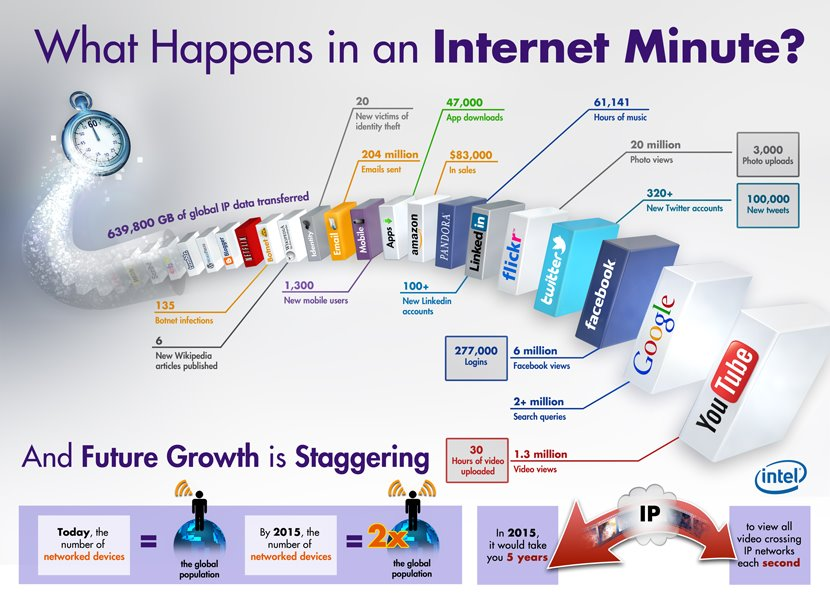
\includegraphics[width=6in]{figures/introduction/intel_oneminute_internet.jpg}
\caption{What happens in an internet minute. (An infographic by Intel\textsuperscript{\copyright})}
\label{fig:intel_oneminute_internet}
\end{center}
\end{figure}

\section{Motivation}
\label{sec:motivation}
% automation and its importance.
% concetrate on collection profiling
% why is it important to know what do we have
% in the collections.
Due to the fast growth and scale of data, the need of automation support in digital preservation processes arises. In order to conduct preservation planning effectively, one has to undertake a well-defined process consisting of numerous steps \cite{Becker:2009fk}. Very important part of this process is the definition of the content that has to be preserved and the representative sample selection. 

The validity and effectiveness of the planning process is highly dependent on a content profile because it defines the scope of the produced plan. A profile defines the content of a collection in terms of its meta data and properties. This meta data plays an important role when preserving digital objects as it not only carries important information about the objects themselves, but also about their structure. Such information provides hints about the digital objects and their type and helps experts decide the best course of action regarding the long-term accesability and preservation of data. A profile also defines a set of sample objects, that are representative to the whole collection of objects. The selected samples provide the basis for the experiments based on which potential courses of action, called preservation alternatives are evaluated. This means that enough valid meta information and knowledge about the content has to be obtained so that only proper alternatives can be chosen. In order to achieve this goal, some very important and necessary steps that provide valuable input to planning have to be undergone. These are currently not always done efficiently, if done at all. For example, the content has to be characterized and all the meta data that is extracted has to be aggregated and analyzed before all potential preservation action alternatives can be found and evaluated. Based on this analysis the content that is to be preserved can be split up into homogeneous sub-collections with similar characteristics and significant properties. Furthermore, such an aggregation of the similarities between different parts of the content can enable more efficient stratification of representative samples in an automatic fashion.

%Based on these and on objective trees defined in another step of the process the most effective preservation action is chosen.
%cite objective tree and representatives.

The presevation planning process is currently done semi-automatically and needs much input regarding the content profile from a preservation expert. Due to the scale of the data a preservation expert often does not have a specific overview of the content profile, but rather high-level knowledge, such as ``The collection consists of 1 million audio files''. It seems that many parts of this process, from characterization to plan deployment and execution, can be automated or at least enhanced by machine processes. Also support for large-scale processing and analysis can be provided by distributed architectures and state of the art algorithms. If this is achieved the effect will be much more valuable than the sum of its parts for the Digital Preservation community.

Nonetheless, the current state of the art does not specify a concrete and well-defined way of how content profiling should be done and what information it should aggregate. What is more, there are almost no evaluation possibilities of the results that characterization tools offer. Some tools try to give confidence level, which is a first step towards such a validation, however it is not enough. A simple example of such uncertainties is character set encoding of html files. Many files specify a UTF-8 encoding, however the real encoding used in the file is different. Some tools are able to detect this, whereas others just report the declared encoding. This is only one of many examples of such uncertainties that arise due to missing quality assurance steps during the characterization process. Such seemingly minor pecularities can cause huge impact on the chosen preservation alternative and thus on the final result of the preserved content. The ability to detect them on a larger scale, to find out subtleties and nuances between different objects in a collection and to select valid representative objects will greatly enhance the preservation planning process.

Thus, a specific way of aggregating large amounts of meta data and its multidimensional representation would be of great value. Only with such a content profile efficient preservation planning can be achieved.

\section{Problem Statement}
\label{sec:problem_statement}
Very often collection and content profiling is done on a very high level, that
is often insufficient for a planning process, especially if this process is to be fully automated.
The current state of the art of content profiling in preservation plans is creating a short description, written by a preservation expert. These descriptions are usualy a very high level assertions, such as: ``The collection contains about 2 million TIFF files''. The profile also contains simple metrics, such as (approximate) collection size, and number of elements as well as the formats identified in the collection. 
These measurements are important but are not the only ones needed for the creation of an efficient preservation plan.
For example, the information about the size of the whole collection is not enough. Other size related measures, such as the overall size of all files in a collection that have a specific format, or the average size of files with a mime type 'text/plain' can be much more significant and helpful in a preservation planning process. Another example where simple measures are not enough are the formats within a collection. In cases of heterogeneous content the distribution of the formats in combination of some other property can turn out to be very helpful for analysis and comprehension of the content. Moreover, in cases of format-homogeneous collections the file format alone will play only a minor role. Combining them with other properties such as the creation date or the creating application could however give deeper insight into the collection.
These are only a few of the examples of multi dimensional characteristics that could turn out to be important in content profiling. However, there are many more that will play different role from case to case.

Furthermore, the creation of a plan has very specific requirements. For example, it needs a small subset of the collection in order to conduct some experiments over it. Based on the results, recommendations and decisions about the preservation actions of the whole collection are produced. Thus the choice of a representative collection subset is a very important process, that is unfortunately often taken lightly, e.g. done randomly or done based on a very shallow analysis. Besides of the manual and random choice of samples in current preservation practices their integration within the planning process is also done manually (either by file upload or manual filling of the related sample information).

Currently, there is no tool that meets these planning requirements and tries to tackle and solve problems arising from the large volume of content, the sparse meta data, the conflicts in the measurements and many other.

The rapid data growth introduces even more problems. In the case of web archives for example, much work has to be done in capturing the significant properties of such dynamic content as the World Wide Web, since the harvested content gets outdated almost immediately after the crawl has been done.

\section{Aim Of The Work}
\label{sec:aim_of_the_work}
In this thesis we aim to analyze the requirements for such a content profiling process and to create a well-defined approach to generate and represent it, so that it can be used as input to other tools, e.g. preservation planning and preservation monitor components.

This will provide a strong basis for preservation planning experts and processes as well as set the foundation for experiments with reduced bias.

The architecture of a software tool that is able to read the characteristics of large amount of files and generate a content profile is to be designed as well as a prototype to be implemented. 

\section{Methodical Approach}
\label{sec:methodical_approach}
In a first step a research of the current methods in scientific projects and institutional practices regarding content profiling will be done. Based on this, a short analysis of the existing gap between the idea of content profiling and the actual steps done will be carried out. 

The main part of the thesis will be the creation of a specification and the architecture of a software tool that is able to profile larger amounts of data and produce output conforming to that specification. In the next step, research about applicable algorithms able to find a (representative) subset of a given collection of characterized digital objects will be performed, and a prototype implementation will be created for the content profiling tool. 

Afterwards a use case study will be conducted, where the produced prototype will be applied on a the Open GovDocs1 collection provided by the Digital Corpora for scientific experiments, which consists of nearly 1 million files and has a total of almost half a terabyte. 

In the last step an evaluation of the tool and the methods applied will be done and based on it a conclusion will be drawn.

\section{Structure Of The Work}
\label{sec:structure_of_the_work}
This thesis is structured as follows: The next chapter offers an overview of digital preservation and preservation planning. The state of the art regarding content profiling is summarized and some observations of the author about the the current related work are discussed. In Chapter 3, a theoretical view of content profiling is presented, where its requirements, issues and open challenges are discussed. Chapter 4 presents the architecture and gives deeper insight into a prototype tool that is designed and implemented as part of this master thesis. The following Chapter 5 describes a use case that was conducted in order to evaluate the tool and draws conclusions about the content profiling approach proposed in this thesis and its implementation. In the last chapter a summary of this thesis is provided as well as the open issues and next steps regarding content profiling that have to be undertaken in future research.

%%%%%%%%%%%%%%%%%%%%%%%%%%%%%%%%%%%%%%%%%
\chapter{Digital Preservation \& Preservation Planning}
\label{ch:relatedwork}
%%%%%%%%%%%%%%%%%%%%%%%%%%%%%%%%%%%%%%%%%

\section{Preservation}
Currently, more and more information is produced in digital form and more and more information has only a digital representation. This has enourmous implications for national and state archives, libraries, scientific institutions and business enterprieses but also the small companies and even private people as they often face data corruption and access problems in the long-term.
In general, digital preservation (or DP for short) copes with two main problems; preserving content (bit streams) for longer periods of time and ensuring these contents are accessible and understandable in the future. When talking about ``the future'' or ``longer periods of time'' we mean ``as long as the content is needed''.
Of course this view is over simplified and there are many more challenges in digital preservation. From the fundamental technical problems through organizational and social challenges to practical and financial ones.

A good example to picture the problem and challenges in DP is presented in \cite{Lorie:2001:LTP:379437.379726} and in \cite{Rauber:2009:dpchallenges}. Imagine a file created today on a specific physical machine. This file is nothing more than a series of bits shaped in a specific format. In order to access this file in the long term, not only the bits and bytes have to be preserved but also the way of interpreting them (the format specification). This would also require to preserve the programms that can open, render and manipulate the file, which in turn will require the preservation of the dependency libraries and software packages as well as the operating system and the whole environment in which these programms or programm versions run. Failing to preserve only one single part of this chain and the file would be lost (even if the physical bit stream is still in tact).

Due to this and many other problems a community of preservation experts has emerged. Through the last decade a number of DP-related research projects have been conducted that have identified problems and treats and have advanced the state of the art in this filed. An overview of the EU DP projects and activities is presented in \cite{strodl:2011:dpreport}. Starting in the mid nineties scientists recognized that these problems could lead to disasters and thus the need of digital preservation and its importance. By the beginning of the new millenium there were the first initiatives and projects in the EU that started focusing on research topics related to DP aiming the establishment of a community, identification of target groups and transfer of expertise (ERPANET\footnote{http://www.erpanet.org/}, DELOS\footnote{http://www.delos.info/}, DPE\footnote{http://www.digitalpreservationeurope.eu/}). The first scientific research was focused on topics such as standards, system concepts, selection and appraisal policies and fromat identification. Afterwards more technical and practical approaches were undertaken to research the preservation of simple digital objects such as office documents and images (PLANETS\footnote{http://www.planets-project.eu}, CASPAR\footnote{http://www.casparpreserves.eu}). All this helped the establishment of a solid community and a body of expertise.

Present initiatives include more fundamental research that tries to focus rather on more complex and interactive objects than simple and documents and data structures. Projects such as LiWA\footnote{http://www.liwa-pro ject.eu} attempt to solve issues related to Web Archiving whereas projects such as TIMBUS\footnote{http://timbusproject.net} and WF4Ever\footnote{http://www.wf4ever-pro ject.org} focus on the preservation of business processes and scientific workflows.
Other projects such as SCAPE\footnote{http://scape-project.eu} build upon the solid framework established in the past and aim to improve the state of the art of DP by developning infrastructure and tools for scalable preservation actions and integrating them with automated policy based preservation planning and preservation watch systems and workflows.
%what does the future hold

\subsection{Most Common Approaches}
% the tools at hand, why are these important, trade offs
Through the years many tools and procedures were developed in order to preserve digital content. In the literature there are often different names for the same concepts. Here we present the most prominent ones. \newline

\textit{Bit-Stream Preservation}
is the concept of copying the bits to a different medium with a different (physical) location. There are many different media, which can store digital data. Some are more stable than others, some are more popular than others. No matter on what type of medium is chosen for data storage, CDs, DVDs, HardDrives, etc., it is not guaranteed that the data stream is safe. Through physical damage, bit rot or other disasters, there is a high chance that your digital storage media will fail to reproduce your bit stream. Thus on this lower level the only option would be to copy the streams to a different medium from time to time. This is strategy is often referred to as \textit{refreshing} \cite{Lee:2002:SOTADP}.

However, refreshing the data does not guarantee that it will be accessible in a later point in time as new media are also error prone. Therefore, approaches like LOCKSS (Lots Of Copies Keep Stuff Safe) \cite{reich2001lpw} make use of the distribution of many independent copies. Developed at the Stanford University the LOCKSS approach was implemented in a librarian software system that deploys many low cost copies of persistent web-caches and enables the detection and repairment of damages based on voting in opinion polls \cite{Maniatis:2003:PPR:1165389.945451}.
%eventually say other projects that use LOCKSS (ExLibris, JISC, Hoppla, etc.)
Following a LOCKSS approach, however, only minimizes the risk of losing data. If there is no effort spent in management of the copies, then it is fairly easy to lose track of the copies. For a software tool this might seem irrelevant but for a private user this is a real issue. Furthermore, even if enough well-managed copies have been stored and the data stream has been preserved, there is always the issue of software obscolescense and thus failure in the access and interpretation of the stream. \newline

\textit{Logical Preservation} tries to cope exactly with this problem. In order to preserve not only the bit stream, but also to ensure the integrity of a digital object and its successful interpretation in the long-term a migration approach is used \cite{Lee:2002:SOTADP}. New operating systems, new software tools or new versions are sometimes incompatible or unable to render and manipulate older formats. To cope with technology changes, digital preservation often uses a conversion strategy where the data is migrated (moved) to another format that is usually considered to be more stable than the original. A format is considered worthy and stable for preservation purposes when it is standardized, the format specification is open and well-documented, there are no patent owners and license fees that apply. The Florida Center for Library Automation, for example, offers a report\footnote{http://fclaweb.fcla.edu/uploads/recFormats.pdf} with the recommended data formats for preservation purposes that is considered as a good reference and starting point. However, there is no ultimate reference table or no ultimate file format that fits all preservation purposes. From use case to use case different aspects have to be considered. Neither standards, nor migration tools alone can ensure that a digital document remains accessible and its integrity remains unharmed. Wing and Ockerbloom further discuss the topic as they analyse what information is preserved by type converters and formalise the notion of respectful type converters in \cite{859529}. Informally a migration tool (or a converter) respects a certain type T if an original object A and a converted object B show the same behaviour when viewed as objects of type T. Rothenberg gives a good overview of common flaws of theconcepts of logical preservation in \cite{rothenberg:1999:ensuring} and summarizes important aspects that should be considered in DP. 

Nonetheless, logical preservation is often applied within digital preservation systems and repositories. As it also has potential pitfalls, it is not to be taken lightly.
Another more practical downside to migration are the storage costs. Often the target format has a bigger footprint than the original. Also the conversion of huge amounts of data is an error prone process that is not easy to validate \cite{Lorie:2001:LTP:379437.379726}. Furthermore, if the migration path consists of several steps one has to make sure that all required meta data of the original is also migrated to the new versions of the objects. Another related issue is also quality assurance. As it is infeasible to check manually if the conversion process was successful, there are very specific requirements and processes that have to be followed in order to automate the verification of the preservation action \cite{feng:2010:qrofm}.
All these and other issues have to be carefully taken into account before choosing such a preservation action.
\newline

\textit{Emulation} has the verb ``emulate'' in its root, which means to imitate or reproduce.
In software terms, an emulator is a software tool that imitates the behaviour of a (hardware) system/framework (usually an older one) in order to run other (obsolete) tools that are meant to run on the emulated system. Clearly, this approach can come in handy in some DP activities.
In \cite{rothenberg:1999:ensuring} Rothenberg gives an overview of a process for preservation that is based on an emulation process. The author states that not only the data (bit-stream) has to be stored but also the bit stream of the original program, the operating system and all other necessary parts, e.g. dependencies and used libraries. Also a thorough and complete description and specification of the underlying architecture have to be provided in a form that is readable by potential future emulator authors. If these prerequisites are met, an emulator that mimics the specific hardware needed to run the tool can be created.
Lorie points out in \cite{Lorie:2001:LTP:379437.379726} that the specification of the architecture has to be perfect and complete, which is an immensely difficult task. Another very important argument he makes is the evaluation of such an emulator. Even if all needed input existed and a hypothetical emulator was created, how can its correctnes be proven as no original hardware device exists?

These and other reasons combined form one of the biggest downsides of emulation; cost. The effort, manpower and infrastructure needed to emulate an environment that renders digital documents is often more expensive than the value of the content of the documents themselves.

Nevertheless, emulation is widely used in specific branches, such as video gaming.
Guttenbrunner et al have evaluated different strategies for the preservation of console video games in \cite{guttenbrunner:2008:evaluating} and came to the conclusion that while migration shows very good results for the preservation of visual and audio components it completely fails in interactivity. Emulation, on the other hand, showed promising results. All of these, however, were strongly dependent on the sample objects that were emulated.
%TODO stress more on the last statement

\subsection{Preservation Planning}
Preservation planning is a key task in DP that has to be undertaken by every institution or person that is serious about preservation. Numerous DP related projects have investigated the key requirements and processes involved in preservation planning. Projects such as PLANETS\footnote{http://www.planets-project.eu/} have created very strong fundaments in this area and have developed tools such as PLATO\footnote{http://ifs.tuwien.ac.at/dp/plato} - the preservation planning tool which supports a special workflow and helps users througout numerous steps with the goal of creating a preservation plan. Follow up projects, such as SCAPE\footnote{http://www.scape-project.eu/} advance the state of the art and enhance the planning capabilities by improving the current status, by building up a framework around the process that supports many new features such as preservation monitoring services and by automating the whole process in order to provide a scalable, robust preservation planning process.\newline

\noindent\textit{What is Preservation Planning?}\newline
The OAIS reference model was developed by the Consultative Committee for Space Data Systems and soon afterwards was dubbed to be an ISO standard \cite{iso:2003:oais}. This high-level reference model has proven to be a helpful tool for the DP community for many years. Undoubtedly, one of its key parts is preservation planning.

It is a decision making process that evaluates different preservation strategies or actions and chooses the most appropriate one. This process is highly dependent on object characteristics and institutional settings and requirements \cite{STR07_jcdl}. The goal of the process is to create a preservation plan that documents all the steps and choices that were made, the policies that were followed while making these decisions and the different preservation alternatives that were evaluated. It offers a complete documentation of the decision that allows one to repeat all experiments and verify why a certain preservation action was chosen.

The preservation plan is a very concrete artifact, opposed to policy documents, that specifies an action plan for the preservation of a set of digital objects.
\begin{quote}
A preservation plan defines a series of preservation actions to be taken by a responsible institution due to an identified risk for a given set of digital objects or records (called collection). The Preservation Plan takes into account the preservation policies, legal obli- gations, organisational and technical constraints, user requirements and preservation goals and describes the preservation context, the evaluated preservation strate- gies and the resulting decision for one strategy, includ- ing the reasoning for the decision. It also specifies a series of steps or actions (called preservation action plan) along with responsibilities and rules and condi- tions for execution on the collection. Provided that the actions and their deployment as well as the technical environment allow it, this action plan is an executable workflow definition \cite{Becker:2009fk}.
\end{quote}

%TODO describe more...
\begin{figure}[th]
\begin{center}
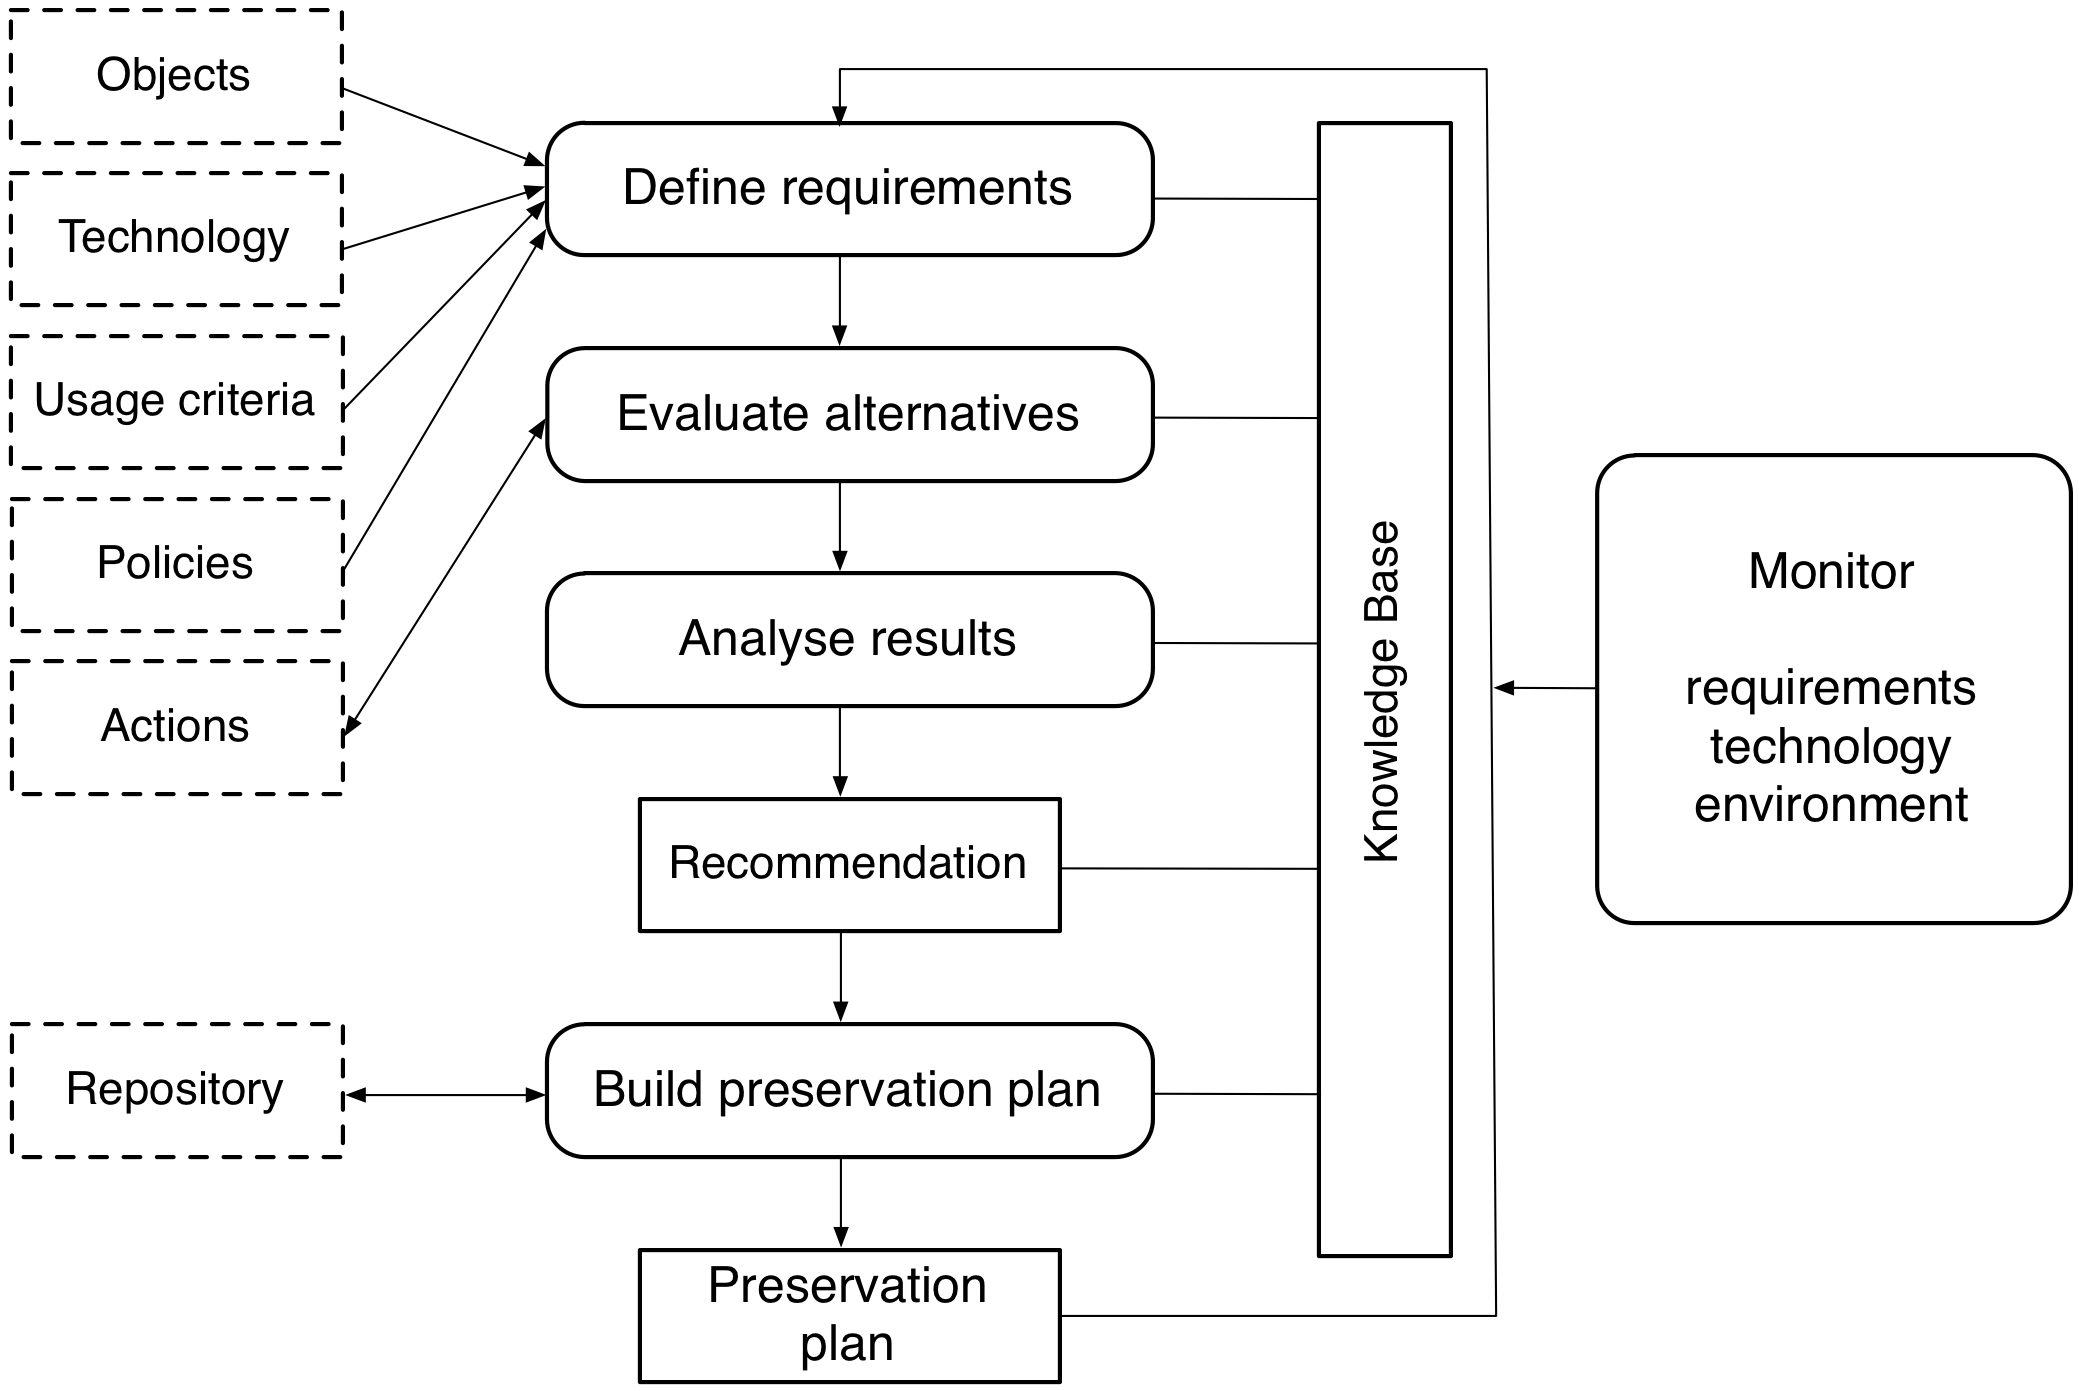
\includegraphics[width=4.0in]{figures/related/planningenvironment.png}
\caption{The preservation planning environment \cite{becker:2010:trustowrothy}.}
\label{fig:planenv}
\end{center}
\end{figure}

PLATO\footnote{http://ifs.tuwien.ac.at/dp/plato} is an online tool developed at the University of Technology in Vienna, which supports the whole preservation planning workflow.
It guides the user through all necessary steps to create a fully documented (and executable) preservation plan. The workflow follows a process specific to a preservation planning environment as the one in figure \ref{fig:planenv}. The process constitutes four main phases: define requirements, evaluate alternatives, analyze results and build preservation plan, all of which are covered by PLATO with respect to the context of the current use case, such as the objects, the current technology, policies, etc.
There is also an external monitoring phase which feeds back important information about relevant changes in the environment, which can cause a reiteration/reevaluation of a preservation plan. A detailed overview and a high level design of such an addition to the preservation planning enviroment can be found in \cite{duretec:2012:watch}.

%A key aspect of a preservation plan is the description of the collection. It includes general characteristics and allows the stratification of sample objects, which are the basis for the experiments and evaluation of the potential preservation actions.


%what it is, overview, steps, Plato, etc.
% the big picture
\section{Collections}
%A collection here is defined as a set of digital objects that was created by some process or a user for some specific reason. Whether all digital objects are stored on the same physical location, how they are managed is irrelevant in this context. It is important to keep in mind that a set of digital objects exists and all of its objects are related for some reason.
In order, to create and analyze a collection or a set of digital objects the meta data for each object has to be examined. Meta data is a structured information about the data (objects) itself. It is usually stored within a file, that provides further information about the content and format of the file as well as other important characteristics. In general, there are three main types of meta data: descriptive meta data for discovery and identification (e.g. title, author, etc.), structural meta data (page ordering, image width and height, etc.), and administrative meta data that helps management of the resource (e.g. creation date, type, etc.). The National Information Standards Organization - NISO\footnote{http://niso.org} has provided a series of articles and reports in order to help people, archivists and experts understand meta data and its importance \cite{citeulike:6387279}.

Today, analysis of such huge content often is done in a manual fashion, which can be a very time-consuming and cumbersome task. If there would be tools at hand that support identification and characterization, data aggregation, filtering, collection splitting, etc., the the analysis process will be automated to a certain degree, hence analysis will be handled much faster and potentially much more efficient. 

It is noteworthy, that content here neither refers to the semantics of the information stored within the digital objects, nor to their visual representation characteristics or anything similar, but solely to the definition of the collection in terms of meta data, such as formats and format-related characteristics.

Consider a collection of digital photographs of old newspapers. Its content here does not refer to the content of the newspapers, but to the meta data characteristics of the images that comprise the collection. The following paragraphs provide more details on metadata and how this refers to content profiling for preservation planning.

\subsection{Identification vs. Characterization}
Based on different properties/characteristics a collection can be dubbed homogeneous or heterogeneous. Usually to a user a homogeneous collection would be a set of files that consists only or mostly of objects having the same format or even the same type (audio, video, text, etc.). This however, is an oversimplification, which has enourmous side effects for preservation planning.

Consider the following example where a collection consists of N digital objects, which share the same extension, e.g. 'pdf'. To a normal user, this would be a homogeneous collection. An advanced user, however, would know that the extension of a file does not really specify the format of the file and thus could assume that there are differences.
One step further would be to conduct an identification process that looks for the specific file format and format version. Assume that in our example 95\% of all files have the same pdf format and format version.  Then this could be considered a homogeneous collection with respect to the format. 
In a next step, however, characterization is conducted and now there are many more properties, such as \textit{creating applicatons}, \textit{encryption}, \textit{password protection}, \textit{tags}, etc.
Regarding these characteristics, the same collection can be considered to be heterogeneous.
Clearly, all of this is very important to preservation planning, since different preservation actions produce different results exactly because of such differences.

Thus the question remains, how to identify such important properties that define the homgenity of a collection? Following this train of thought, clearly the format is a very important characteristic. However, it does not cover all cases (as in the example) and many others are important.
% what is important here
% what is identification, what is characterization.
% meta data, distributions, aggregations, scalability, etc.
% homgeneous vs heterogeneous collections
% some properties are obviously more important than others.
% is the format ultimate significant property...
\subsection{Preservation Analysis}
As collections in DP are often just too large for a human being to comprehend, the meta data provided by identification and characterization has to be aggregated and analysed in some fashion. For this purpose different statistical information is used to understand and stratify  the content into different homogeneous parts. Often simple statistical measures, such as minimum, maximum, average, standard deviation, etc. provide meaningul information about the current content one has to deal with. Moreover, histograms and distributions of mimetypes, formats, format version and other properties help to create the bigger picture of the content that is to be preserved.

Once the bigger picture gets clearer, the collection can be divided into different (more) homogeneous parts, which will ease the decisions that have to be made regarding their future with respect to DP and PP.

Another important part would be finding representative sets within the homogeneous content. These are small sized sub collection (usually consisting of 10 or less sample objects) that are somehow representative to the selected collection or part of it. The representativeness can be determined based on the distribution of different characteristics or combinations thereof. These representative samples form a better suited common ground for the experimentation phase of the preservation planning process. Finding such small subsets within homogeneous collections is potentially much easier than in heterogeneous context. This problem will be investigated in later parts of this thesis.

\subsection{Scalability}
As discussed in chapter \ref{ch:content_and_digital_preservation} content growth nowadays has a tremendous pace. This fact has some serious implications on how information systems have to deal with it. Scalability does not only pose a problem related to volume and performance, but also to usability and presentation, automation and costs.

Looking at the growth of content within web archives, for example, and their projection the problem of vertical scalability becomes clear. Vertical scalability (i.e. installing machines with better performance) will not be able to solve the problem of storage and data management, not to mention the effective analysis of data.

Since this is a problem not only related to digital preservation but to information systems in general, there are many studies for algorithms, technologies and architectures that enable horizontal scalability, i.e. attaching more commodity machines and distributing the payload among them.

Driven by economies of scale and Cloud Computing has played an enormous role in this area by providing a large set of easy to use and access resources, such as hardware, development platforms and services \cite{Vaquero:2008, 4738445}. Distributed Platforms as a Service (PaaS), such as Amazon AWS\footnote{http://aws.amazon.com} and Amazon S3\footnote{http://aws.amazon.com/s3/}, Google App Engine\footnote{https://developers.google.com/appengine/}, Heroku\footnote{http://www.heroku.com}, etc. have proven to be very performance- and cost-effective. Distributed approaches and algorithms, such as Googles Map Reduce \cite{Dean:2008:MSD:1327452.1327492} have found many applications in various fields of computer science. 

Map Reduce is a fairly modern parallelization algorithm for processing large data sets on certain kind of distributable problems. The framework can make use of a large amount of nodes for the computation. It takes as input a set of key/value pairs and produces a set of output key/value pairs. It typically consists of only two functions: map and reduce. In some cases a third finalize function can be used to do some further computation that needs all the results of the reduce steps.

The Map function takes a set of pairs of keys and values in the form of (k1, v1) ant transforms them to a set of intermediate key/value pairs. The framework groups the intermediate values associated to the same key together and passes them for further processing to the Reduce function.

The Reduce function accepts an intermediate key and a list of values associated with that key and is responsible for computing the (partial) final result. The reduce function can be invoked many times by the framework and there is no guarantee that it will be run on the same node as the Map function. This means it has to be idempotent and agnostic to external knowledge about the distribution.

This rather simple approach has been widely accepted by the OpenSource community and was implemented by the Apache Software Foundation in a library called Hadoop\footnote{http://hadoop.apache.org}. The possibility for integration with a BigTable-like Store \cite{Chang:2008:BDS:1365815.1365816} (HBase\footnote{http://hbase.apache.org}) and a distributed file system (HDFS\footnote{http://hadoop.apache.org/docs/hdfs/r0.22.0/hdfs\_design.html}) has enabled many companies to handle the big volumes of data they have. Google was using a similar architecture for its index construction, article clustering and statistical machine translation. Yahoo uses it for spam detection in its mail service and other big corporations use it for data mining, ad optimization and more.

All this implies that analysis of preservation related data should be feasible and cost-effective. Nonetheless, tools nowadays often lack the ability to analyze content on a larger scale, or if they support it, there is a trade off in the analysis depth.

\section{Tool Support}
%talk about meta data tool support
%preservation planning tool support and automation and scalability
%content profiling/ format profiling tool support
%repositories, monitoring services

There are numerous software projects and tools that are related to DP and focus on the field of identification and characterization. In this section we observe some of the most prominent ones. A recent report (created as part of the SCAPE project) summarizes an evaluation framework and the results of the tests of several identification and characterization tools \cite{Knijff:2011it}. It provides a rather good overview of the current state of the art of such tools but concentrates mostly on their identification capabilities. In the report six tools (DROID 6.0, Fido 0.9, Unix File Tool, FITS 0.5 and JHOVE2) were evaluated against 22 criteria among which, the tool interface, its license type, platform dependencies, accuracy of reported results, documentation, etc.

Here we summarize the strengths and weaknesses of these and some other tools briefly.

\begin{itemize}
\item \textbf{DROID 6.0}\newline
Droid is an identification tool produced by the National Archives, which uses the PRONOM\footnote{www.nationalarchives.gov.uk/pronom/} registry and its format signatures and/or file extensions. It provides information about the mimetype, format and format version of a file as long it is in the DROID signature file, which contains the 'magic numbers' of the PRONOM registry. It also outputs a PRONOM Unique Identifier or puid, which can be used to trace the format back into the registry.
Unfortunately, the registry is not open and its maintanence is slow. However, the tool is very useful and widely used within the DP community.

\item \textbf{Apache TIKA}\newline
Tika is an open source project from The Apache Software Foundation that is able to extract metadata from files with various formats. It is a stable tool able to identify files by analysing their bitstream and allows the deeper characterization of some of these files.  

\item \textbf{FIDO 0.9}\newline

\item \textbf{UNIX File Tool}\newline

\item \textbf{FITS} \newline
The File Information Tool Set is developed by the Harvard University Library. It wraps common identification and characterization tools as the ones described here and tries to consolidate them and provide a normalized output. By providing basic provenance information for each extracted record it combines the consolidation result and provides a very basic confidence status for the extracted value of each property. This proves to be helpful for cases where there are uncertainties. The framework is designed to be extended, so that other tools can be also added. The tool seems very helpful, although there are some unstabilities and problematic cases.

\item \textbf{JHOVE}\newline
JHOVE is one of the most well-known identification and characterization tools used by the DP community. It is also developed by the Harvard University Library and is able to extract meta data from various formats based on different modules. Probably one of the most valuable features of JHOVE is the ability the check a file for wellformedness and validity against the format specification.

\item \textbf{JHOVE 2}\newline
JHOVE 2 is a successor project for the JHOVE tool and also provides an extensible architecture for characterization tools and modules. It is developed as an open source tool by the California Digital Library, Portico and Stanford Univeristy. Currently it produces helpful output only for a few types of documents as the different modules are not yet developed.

\end{itemize}

Although this list is not complete, and there are many other tools that are able to extract meta data as well it shows that the current state of the art is able to provide enough meta data that could be used as input for various preservation activities. The tools have their downsides in terms of format coverage and/or performance, but still provide very valuable information.
Currently there are only a few tools however, that are able to analyze collections. PRONOM ROAR, for example, is able to create a format profile within a repository interface with the help of DROID.
Various repositories provide basic information as the formats and size of objects, however no further stratification is possible, although the characterization data is present.

% what is present.
% explain that the tools for different types of contents are there, but no tool does
% collection profiling
% scape evaluation of characterisation...


\section{Quality Assurance}
One of the biggest downsides of all identification and characterization tools is the lack of quality assurance processes. Often there is no way to validate if an extracted measurement value is really representing the truth. This is a huge problem, as it is hard to make assumptions about validity without having a ground truth.
Some tools such as FITS try to tackle this problem on a very basic level by stating a confidence level in the form of an enumeration (OK, SINGLE\_RESULT, PARTIAL, CONFLICT). It is not perfect, but it provides the user with warnings about potential threats.
A big problem here is the consolidation. Often tools provide the same measurement for a specific property but the output format is different. This makes it hard for an automatic consolidator to decide if the values are equal or not. Thus the problem of quality assurance depends on external information provided by other processes or even by manual verification. 
Clearly, this is a hard, tedious and long running process and thus it is (partially) neglected.
Nonetheless, it is an essential precondition in order to assure correct input data for the analysis.
% despite the tools there is a big gap
% tools extract some measures, but there is almost no way, to assure that
% a measurement is correct
% often tools extract the same information and represent it in different way, thus providing a conflict - verification is hard...
% JHove validation, verification


\section{Observations}
In order to prepare a preservation action plan some prerequisites have to be met. The following provides a simplified list of steps that would occur in a common digital preservation scenario, usually in the following order: 
\begin{enumerate}
\item Organizational policies about the management of the content are created and curated.
\item A monitoring component is used to observer the policies and operations over the content for violations.
\item As part of the repository ingest an identification and deep characterization process extracts valuable meta data and stores it within the repository.
\item A content profile is generated and exported for other tools.
\item A monitoring component identifies that a certain subset of objects violates the policies and notifies a planning expert for the potential threat.
\item A planner uses the content profile, a profiler to analyse and stratify the content into smaller homogeneous partitions as well as identify representative sample objects for the partitions.
\item A planning tool is used to validate the threat and to create an action plan that is able to cope with the policy violations.
\item The action plan is submitted to a repository, which knows how to execute the described preservation action.
\item The monitoring component observes the operations of the repository and notifies the interested parties of important events, such as throughput, failures and task executions. 
\item The violation is taken care of and the monitor component continues its work.
\end{enumerate}

The state of the art provides some of these components and actors in this high-level workflow. Any organization, which is serious about digital preservation has its own set of policies of how to handle different types of content. The problem here is that often such policies are just high-level descriptive statements, which are not structured in any specific form and thus are not machine readable. This makes it almost impossible to use in automated fashion. Also there are numerous repositories that can manage digital objects and extract meta data from them. The planning tool PLATO provides the needed facilities to create an action plan.

However, a couple of components are missing. A preservation monitor, that scans relevant properties of the world and evaluates their values for changes, eventually notifying users or other agents of interesting events. Such a monitor is currently developed within the SCAPE Project (TODO cite).
Another crucial part that is missing is a tool able to profile a massive content set and stratify it into smaller homogeneous and managable partitions. If there was such a tool it would provide two main benefits. First, easier analysis and content stratification and thus better foundation for planning experiments with reduced bias and second input to a preservation monitor that will be able to create a global profile of content, which would be of great benefit to the DP community.

% summarize, what is going on,
% what is missing
% what is the problem of the current state of the art
% based on the research you made.

%%%%%%%%%%%%%%%%%%%%%%%%%%%%%%%%%%%%%%%%%
\chapter{Content Profiling}
\label{ch:contentprofiling}
%%%%%%%%%%%%%%%%%%%%%%%%%%%%%%%%%%%%%%%%%

\section{Preservation Planning}
%what is missing - CP
	%why does pp not work without cp
	%try to invert the big picture and state that cp is the actual thing and pp just does not work 	without it
% representative set is critical

\section{Collection \& Content Profiling}
% goals
% what is it c3
% jhove (identify, characterize, validate)
% why is it important (iteration of before)
% specification (representation, xml, rdf)
%...

\section{Representative Sets}
% what is the problem,
% how do we create them/find them
% ...

\section{Continuos Profiling}

%%%%%%%%%%%%%%%%%%%%%%%%%%%%%%%%%%%%%%%%%
\chapter{C3PO - A Profiling Tool} %change this?
\label{ch:c3po}
%%%%%%%%%%%%%%%%%%%%%%%%%%%%%%%%%%%%%%%%%

This chapter summarises the goals of the content profiling approach discussed so far and gives a detailed overview of the architecture for a prototype implementation of it. First a high level design is discussed and then detailed explanation of the chosen technology, implementation details, enhancements made and trade-offs is provided. Following some algorithms for representative sample selection that were implemented are presented and discussed. At the end a short summary and overview of future interesting work which will enhance the tool and help preservation experts even more in their endeavours is given.

\section{C3PO in Perspective}
As part of this thesis, a software prototype is developed that aims to tackle the issues, problems and gaps presented in the previous chapters. The aim is to create a tool that is able to automatically generate a content profile of large collections (consisting of hundreds of thousands, or even millions of objects). This means a framework that provides enough scalability to be feasibly applied on the metadata of collections of multi-terabyte ranges and beyond.

This profile includes a descriptive statistical representation of the content in the collection, meaning that it contains very specific data such as count of objects, overall size of objects, etc. Furthermore, it provides different visualisations of different aspects of the content, such as the file formats, mime types and many other characteristics and combinations thereof that are of interest to the user of the application.

As presented in section \ref{sec:goals} on page \pageref{sec:goals} the tool that implements the presented approach should fulfil the following requirements.

The user should be able to aggregate large sets of meta data with minimal effort in an automated fashion. The presented approach should be able to scale to million objects and should be ready to pass this threshold by making use of a distributed infrastructure and architecture.

Furthermore, clients of the application (users, or other systems) should be able to obtain a machine readable description of the profile, that contains enough information for the client to obtain a rough overview of the content at hand. This profile has to include the identifiers of a small set of objects that are representative to the whole collection as described in section \ref{sec:representative_sets} on page \pageref{sec:representative_sets}.

Since this overview might not be enough for a planning expert, she should be able to visualise interesting aspects of the content and filter it based on chosen characteristics. As it is unlikely that a single tool can satisfy all possible analysis requirements that an expert might have, it is very important that the raw data or a subset of it is exported in some intermediary format. This will allow further analysis conducted with other software, that might potentially result in even more interesting findings. 

%On top of that a service layer enables the user to query the tool in order to gain a deeper insight into the content. This may include the filtering of the content based on different characteristics and splitting it into buckets, which will allow to compare homogeneous parts (based on one or more characteristika) in an otherwise heterogenous content. 

%Visualizations and multi dimensional representations of these filterings enable to user to understand the profile and thus provide her with the fundamental knowledge and a more stable ground to take more efficient decisions.
The prototype implementation of the profiling approach is called '\textbf{C}lever, \textbf{C}rafty \textbf{C}ontent \textbf{P}rofiling of \textbf{O}bjects' or \textit{c3po} for short and is discussed in detail in the following subsections.
% idea
% overview
% part of scape, watch source, etc..

\section{Architecture}
In this section an overview of the architecture of c3po and its more important aspects are presented. Afterwards, detailed information about the design and implementation is given as well as a discussion of the decisions made is done. The implementation was carried out into two iterations which are presented after the overview.

\subsection{High Level Overview}
C3PO is separated into different modules and provides a relatively simple workflow that follows the three steps of content profiling as presented in \cite{petrov-ipres2012} and discussed in section \ref{sec:content_profiling} on page \pageref{sec:content_profiling}. In the first part it gathers raw meta data and parses it in order to normalise it into a simple internal data model. In the next step the data is cleaned up, partially aggregated and stored into an external to the tool database. 

All this offers the baseline for the deeper analysis provided by some of the modules of the framework. Figure \ref{fig:architecture_highlevel} presents the high level architecture and c3po's modules in a stack diagram which are detailed in the following subsections.


\begin{figure}[t]
\begin{center}
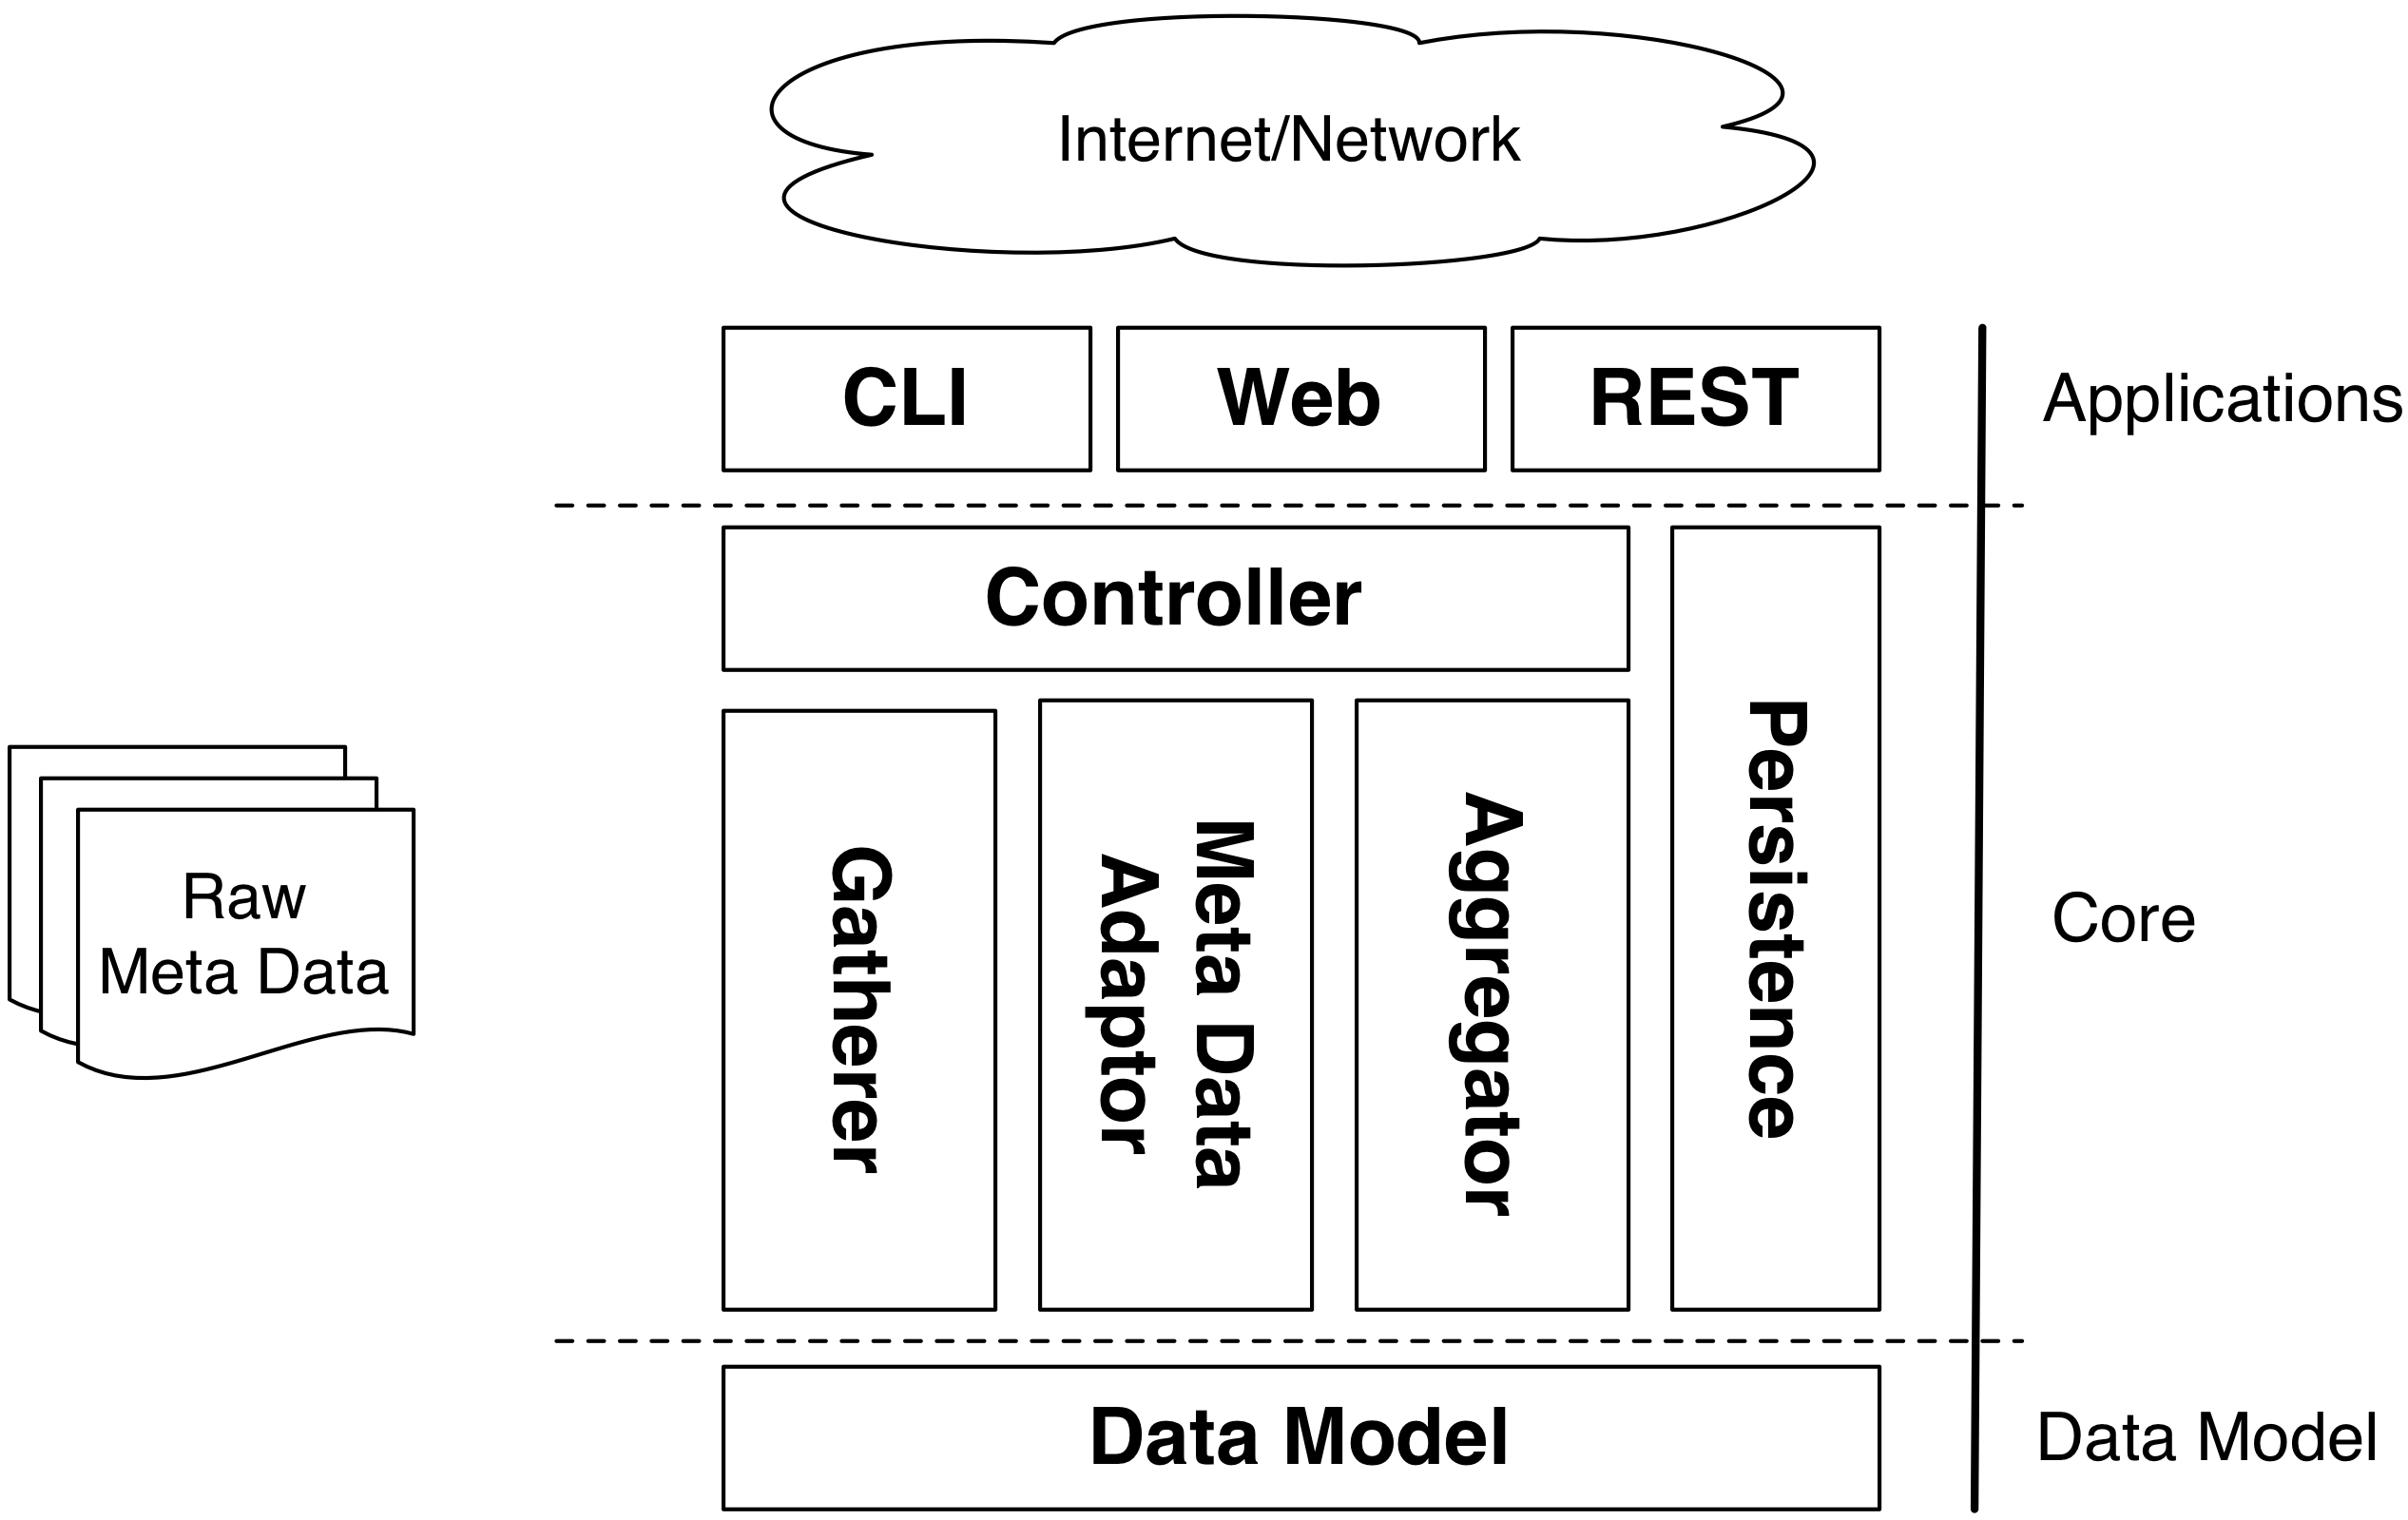
\includegraphics[width=5in]{figures/architecture/c3po_highlevel_architecture.png}
\caption{High-level architecture of c3po.}
\label{fig:architecture_highlevel}
\end{center}
\end{figure}


\subsubsection{Data Model}

At the bottom there is the domain model module which sits as the foundation of the architecture. It represents a simple model that captures the important aspects of the content meta data in a generic way, but still provides the ability to do flexible queries over the data. It consists mainly of elements, properties and values. Elements encapsulate a digital object and capture important information, such as the identifier of an object within its source (e.g. a digital repository), which is important for later access. Properties define characteristics of a given object. These may include information, such as size, format, format version, etc. The values capture measurements of specific properties that are provided by different tools.

\subsubsection{Core}
Above the data model is the main part or the core module, which encapsulates the framework that allows the gathering, normalising and aggregation of the data. It not only offers interfaces that allow the extension of the framework, but also provides the glue-ware to create and run the work flow.

The core wraps the middle part of the architecture stack diagram. It is divided into three logical parts: A controller, sub-components and a persistence layer.

The controller is responsible for chaining the sub components and carrying out the whole workflow of the system.

The three sub-components (Gatherer, Meta Data Adaptor and Aggregator) divide the work and encapsulate important steps of the whole workflow. As described in section (TODO cite) the raw meta data of the content can be stored in many different places or sources. For example, it can be provided locally, in form of files stored on the local file system, or remotely. The remote source can have many different variations. E.g. there can be a remote ssh server that stores the raw meta data again in file form, or a remote web archive server that stores the meta data in special container files called arc (archive) or warc (web archive) file, but there can be also a remote repository, which not only stores the original content but all the meta data for each object in a different way (internal data store, to its local file system, etc.). The latter represents the most likely use case in a real world digital preservation scenario, however all others are possible as well, not to mention that they are easier to use for experimentation purposes.

As the users of c3po should not be interested in the way of how and where the meta data is stored, the gatherer component offers an interface that abstracts this issue.

Since different sources can use different characterisation tools and different characterisation tool outputs, the Meta Data Adaptor component is responsible for instantiating and assigning a specific implementation of an adaptor that can handle the gathered meta data records. 

The last part of the core module is the persistence layer, which abstracts the connection to the external data source, where all raw meta data is stored. It provides interfaces for retrieving the meta data, storing aggregations and analysis results.

\subsubsection{Applications}
On top of the Core module, there are two user applications. One of them has command line interface (CLI) and the other a  web application user interface. This separation has been done in order to optimise network overhead during initial data processing. The CLI application can be executed near the data (e.g. on the same infrastructure as the repository) and can process and store the data there. This near-data processing allows the reduction of network overhead and the utilisation of resources. The web-application on the other hand can be deployed on a different infrastructure and provides interfaces for analysis and representation of the data.

\subsection{First Iteration}
The first iteration was done in order to explore the problem and find out potential issues early on. It was a horizontal prototype and concentrated on the lower levels of the framework.

\subsubsection{Data Model}
As relational databases have stood the test of time and are proven to work in virtually any use case, the natural thing was to try a relational model first. Figure \ref{fig:old_datamodel} shows a simplified version of the key domains of the first data model used. It models the key concepts for generic key value structure in a relational database, which would fit the needs of the collection profiler and leaves out some fields and helper classes. 

The \textit{Elements} describe the digital objects. Each element has a number of \textit{Values}, where every value is a measurement for a specific \textit{Property}. Properties are specific characteristics, such as format, size, or number of pages in a document, etc. 

There are different typed values for the different data types, such as String, Bool, Numeric, Float and Array, which are not shown in the diagram. Furthermore, each value has a \textit{ValueSource}, which provides provenance information.

Although this model was so minimalistic it was proven to be incapable of a high enough performance when querying more specific information (a mixture of more properties and values) due to the generic nature of the Values. This proved to be a big problem in regard to the sparse matrix export requirement (A matrix over a number of properties for each element). This use case provides the user with a great overview of the data and enables her to find important aspects that would otherwise easily evade. Since the data is sparse it was not feasible to query the described matrix of the data in an efficient way, which made the implementation of this key requirement hard.

The underlying data store was a PostgreSQL data base, which is one of the best open relational databases at the time of writing. However, the limitation of the high number of JOINS for the sparse matrix use case is just contradictory to the paradigm, since there is a general rule of thumb that more JOINS result in a poor performance. Through data model enhancements and optimisations and a lot of query optimisation it probably would have been possible to use a relational model effectively. However, this was not the focus of the work, so a new approach had to be chosen.

\begin{figure}[t]
\begin{center}
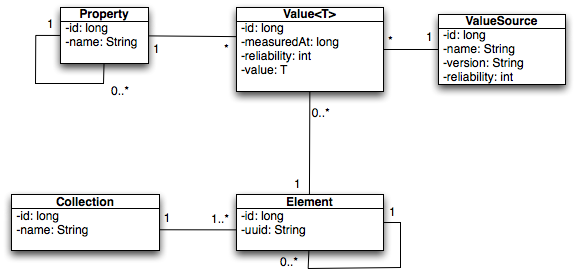
\includegraphics[width=5in]{figures/architecture/old_datamodel.png}
\caption{Old datamodel used in the first iteration.}
\label{fig:old_datamodel}
\end{center}
\end{figure}

\subsubsection{Core}
In the first implementation the controller worked in a single threaded, sequential manner due to simplicity reasons. However, preliminary experiments have shown that some tasks, such as meta data parsing make only partial use of the system resources at hand. For example the cpu utilisation was mostly less than 25\% during data parsing and storage. This was an indicator of a possible enhancement that might result in a significant speedup.

Because of the XML representation of the FITS meta data a parser had to be written in order to adapt the meta data schema of FITS to the internal data model. As FITS files usually are small in size (up to 5KB) the parser that was implemented utilised a DOM based approach. Early tests over a small set of FITS XML files seemed to have feasible performance. However, the first test over larger collections revealed the next issue: memory usage. Even though the amount of objects that had to be created by the DOM parser for each node in each xml document was not so high, the garbage collector of the JVM seemed to be unreliable and the overall consumption seemed to increase constantly with the xml document count and the collection size. This revealed the next potential optimisation.

C3PO's persistence layer was based on the Java Persistence API\footnote{http://docs.oracle.com/javaee/6/tutorial/doc/bnbpz.html} (JPA 1.0) with Hibernate\footnote{http://www.hibernate.org/} as the persistence provider in the first iteration. The higher level abstraction was done via a couple of generic data access object (DAO) interfaces, which were implemented by the client application, and client modules.

This design was chosen in order to allow each client application to choose its own implementation of the persistence layer. This was important since c3po is meant to be deployable in application server containers, that support the Java EE technology stack. For this, a special container managed transactional model would have been needed. On the other hand, content profiling is a data intensive process which can gain from the fact that the tool can execute near the data. That is why, also a local transactional model was needed, in which the tool should run locally near the data without any application server. All this would allow the separation of the data gathering and the data analysis parts of the work flow. The fact that the data base is external to the tool also means that it can be setup near the data or on a specific storage sever that has enough resources at its hand to handle the load.

Using an ORM framework, such as Hibernate is often very useful. However, in this instance a lot of optimisations and tweaks had to be done in order get out the most of the data base. While this was certainly possible, it was not the focus of the work to fight the framework. Using JVM profiling applications, revealed that a lot of resources are used during storage, because of the high volume of data and it seemed the ORM framework was the bottleneck.

\subsubsection{Applications}
In the first iteration only a prototype of the CLI application was implemented that made use of the non-transactional persistence model. It was used to measure performance and to monitor the behaviour of the whole framework. As far as the web application was concerned, only the persistence layer interfaces were implemented in order to validate the design and the separation of concerns.

\subsection{Second Iteration}
This section gives an overview of the implementation changes and enhancements in the second iteration and discusses the benefits and drawbacks of the alternatives.

\subsubsection{Data model}
After examination of the data at hand it seemed that the key value structure was fitting, but through the data base normalisation, performance was compromised. Thus, it seemed appropriate to exchange the underlying data source, which made it possible to remove the ORM framework at all. Its overhead was proven to be unnecessary during meta data adaptation and storage. Also, the analysis of the data seemed to take a unnecessary long time due to the many JOIN operations. One could argue that these could have been avoided by making the data model more specific, however this would have compromised the flexibility, which would have been a huge trade off.

For these reasons the data model was analysed again and different storage possibilities were evaluated.  Due to the natural key-value structure of the meta data it seemed that a key value store would possibly provide better solution to the problem. However, usually such solutions are used for caching (EHCache\footnote{http://ehcache.org}, Memchahed\footnote{http://memcached.org}, etc.) and architecture designers often have problems fitting their data model when such technologies are used for more than their purpose - caching. There are some implementations of data bases that offer most of the flexibility of the relational paradigm, high performance due to their almost key-value paradigm and out of the box horizontal scalability.

MongoDB\footnote{http://www.mongodb.org/} is a document store that uses BSON\footnote{http://bsonspec.org/} (Binary JSON) in order to store documents. These documents can have any kind of structure and do not have to be normalised in the relational database sense. On top of that MongoDB provides native facilities for executing Map Reduce \cite{Dean:2008:MSD:1327452.1327492} jobs on the server, which were proven to be very useful for aggregating and filtering the data. 

As any NoSQL solution, MongoDB does not gain from the fact that the data is normalised and relational. On the contrary, NoSQL solutions often give up normalisation in order to enhance performance of specific use cases. The data model from the first iteration was transformed into three collections (here the term collection is used in the sense of a document store and can be understood as the equivalent concept of a table in a relational database): one for the elements, one for the properties and one for the sources. The values are embedded into each element document and thus each document represents a self-contained object with all its known meta data - values, sources and conflicts. This has one big advantage when querying, as all values are already present without a need of joining the property table. Furthermore the equivalent of a SELECT statement in MongoDB does not retrieve the actual data, but only a cursor over it. This lazy-loading mechanism comes in handy in numerous use cases of the applications.
Figure \ref{fig:document_structure} gives an overview of the basic structure of element documents in BSON syntax. Note that the syntax is very similar to JSON, but provides data type support (e.g. the ObjectId).

Since Map-Reduce jobs are supported natively in MongoDB, it is easy to aggregate specific values of a specific keys in every element document or to execute some analysis queries. Another great advantage of this implementation is the pagination support. Every query in Mongo DB returns a cursor over the data, instead of the data itself. This makes navigation over the data within an application fast and efficient in terms of memory, as one does not have to consider the volume of the queried data.
The third reason, why Mongo was chosen, was the automatic load balancing used by the document store server. The document store supports horizontal scaling and auto node balancing out of the box, which might turn up useful when considering the amounts of data that the profiler has to deal with. To summarise MongoDB was chosen because of the:

\vbox{
\begin{itemize}
\item Natural fit of the data into a key-value schema
\item Native Map-Reduce support for data aggregation and near data processing
\item Query cursor and pagination
\item Horizontal scaling and automatic node balancing out of the box
\end{itemize}
}

\begin{figure}[!htb]
\begin{center}
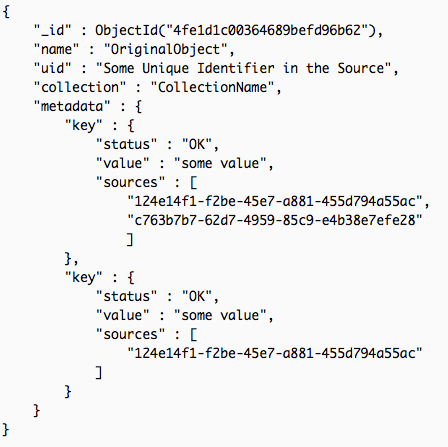
\includegraphics[width=4in]{figures/architecture/document_structure.png}
\caption{Structure of a c3po element in BSON.}
\label{fig:document_structure}
\end{center}
\end{figure}

\subsubsection{Core}
In the second iteration the controller and the meta data adaptors were reimplemented to follow a master-worker pattern.
The controller uses the gatherer interface to traverse the raw meta data files and spawns an adaptor worker thread for each file that has to be processed. This change resulted in much larger utilisation of CPU resources. Each meta data adaptor runs in a thread and is responsible for parsing meta data files that conform to a specific meta data schema. The c3po prototype makes use of a single adaptor for the FITS output format as described in (TODO cite). 

The parser implementation of the FITS adaptor was also changed due to the previous performance results. This time a SAX based approach was used. The Apache Commons Digester library\footnote{http://commons.apache.org/digester/} provides a special SAX parser that traverses each document only once and does not require the building of a complex DOM tree. This results in a much faster parsing with significantly less memory resources.

\subsubsection{Applications}
The CLI application was modified so that it reflects the changes of the new persistence layer.

Since the technology stack was different (no need of JAVA EE) and there was no need of transactional persistence model a new approach was also chosen for the web application. It makes use of a popular web application framework, called PlayFramework\footnote{http://playframework.org}, which does not rely on a complex technology, such as EJBs. It supports the developer to follow the MVC pattern and allows the rapid development of a REST \cite{Fielding:2000:ASD:932295} interface. REST was chosen for two main reasons. For one, it is easy to understand and pretty straightforward to implement. This allows easy integration with other tools, such as monitoring services (TODO cite) and a variety of client applications. The second reason is that other technologies, such as JavaServer Faces Technology\footnote{http://www.oracle.com/technetwork/java/javaee/javaserverfaces-139869.html} (JSF) and Enterprise Java Beans Technology\footnote{http://www.oracle.com/technetwork/java/javaee/ejb/index.html} (EJB) would have meant that only a few application servers will be compliant and able to support the application.
%REST cite: http://www.ics.uci.edu/~fielding/pubs/dissertation/rest_arch_style.htm

The UI was implemented with the help of the framework, by utilising Scala templates and standard technology such as HTML5, Javascript and CSS3. It enables the user to select her collection and obtain deeper overview by filtering the data based on specific properties and values as shown in figure \ref{fig:web_app_overview}.

\begin{figure}[tbp]
\begin{center}
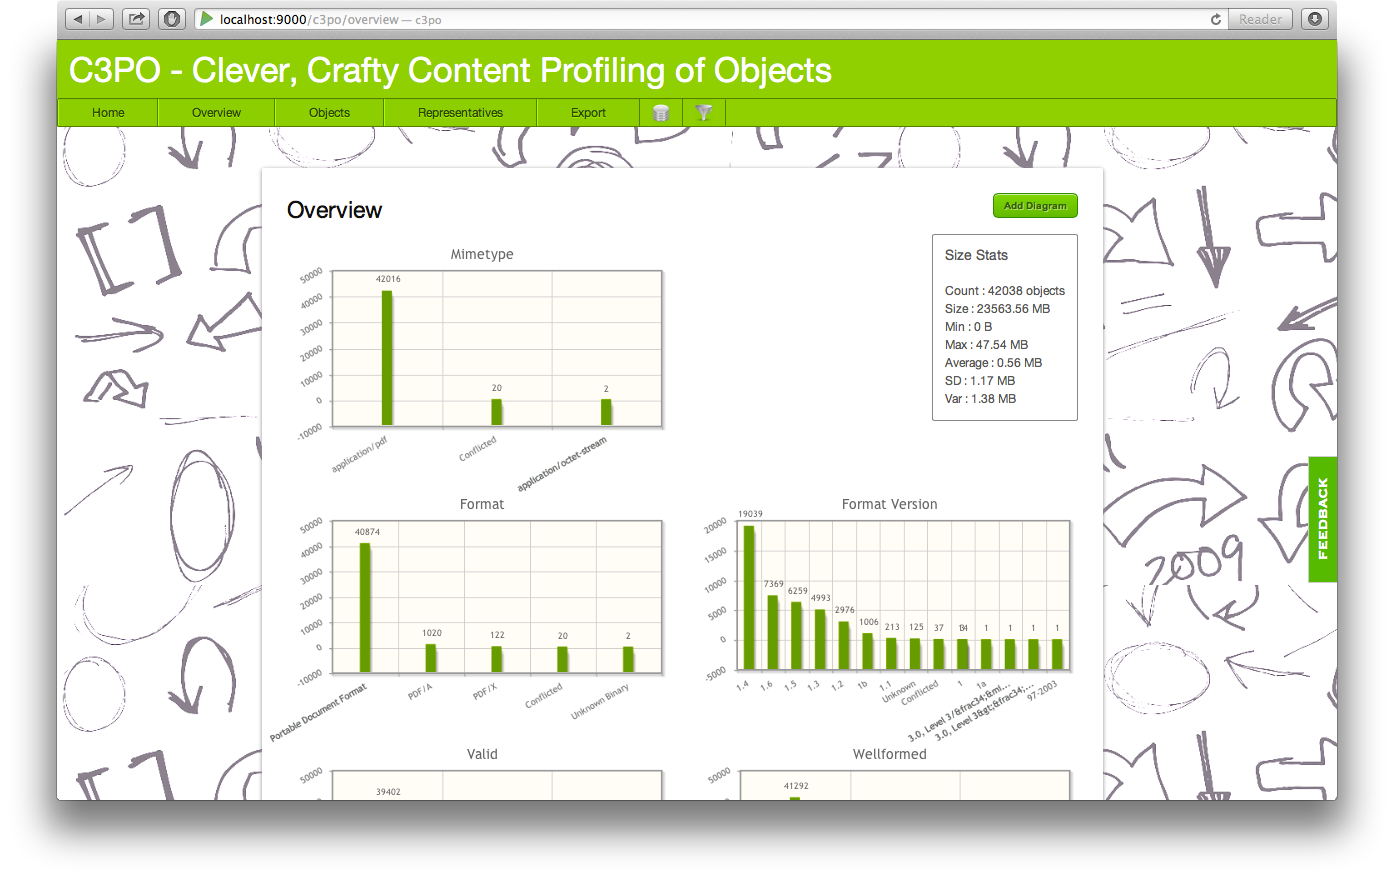
\includegraphics[width=5.5in]{figures/architecture/web_app_overview}
\caption{Screenshot of c3po - Overview of a collection.}
\label{fig:web_app_overview}
\end{center}
\end{figure}

\subsection{Comparison and Results}
Due to the changes made in the second iteration significant performance and scalability optimisations were achieved.

The change from a DOM to SAX parser not only improved the scalability of the system during gathering and parsing, but also improved the time for processing files. With the DOM solution in a single thread environment 1000 files were processed in about 3 minutes on average, whereas with the SAX solution 1000 files were processed in about 15 seconds.

In addition to the SAX parser enhancement the multi threading enhancement also showed promising results. With a single thread, parsing a collection consisting of about 1 Mio heterogeneous meta data files was done in about 165 minutes, whereas the same collection was processed on the same machine with 8 threads in about 104 minutes. This results in more than 35\% speedup just for parsing.

Other test results have shown that parsing and storing the raw meta data for a collection of about ~550 thousand files (web meta data) was done in about 17 minutes on a laptop, whereas the old solution needed about 12 hours for the same set of files on the same machine, due to the overhead of the ORM framework.

Furthermore, exporting a sparse matrix of all property values for every element in the collection was proven to be much faster. This was due to the fact, that the internal representation of the data needed no JOINS anymore and can be done by single iteration over a database cursor.

Many of the analysis queries were changed to be done by map-reduce jobs. Since these run near the data and not in the application itself, the scalability of such queries was significantly improved.

\subsection{Interfaces and Extension Points}
In order to extend the system, the framework provides a couple of interfaces. One important extension point for later use is the GathererInterface which provides an abstraction for the source of the raw meta data. It exposes a unified interface allowing the Controller to obtain streams to the next N files that have to be processed. This design allows a transparent view to the other modules in the system. The prototype of c3po provides an implementation only for local file systems. However, extending it to fetch data from a different source is just a matter of implementing a single interface, which is able to count the files to be processed and to open streams to the next N files. It is up to the implementing class to decide, whether the data will be retrieved over the network and the stream will be passed directly for further processing or it will be cached in batches to the local file system. Depending on the use case both could make sense and thus it is left in the responsibility of the service provider.

Clearly, meta data representation is another important aspect in such as system. For the prototype FITS was chosen, due to it benefits regarding normalisation and conflict detection. Nonetheless, other formats can make sense in specific use cases and when integrating with different sources, that utilise different meta data schemas. In order to extend c3po, one has to implement a simple adaptor that is able to parse the the new schema and return the data in a way that fits c3po's data model. A drawback here is that this will potentially break the property normalisation. For example two different meta data schemas can have two different property names with the same semantical meaning. There are a couple of solutions to this problem, which are taken into account in the design, but are not implemented due to insufficient information of real world scenarios. The first, could be to provide the mapping between these colliding properties via some user configuration and to take them into account during parsing or post-processing. The second solutions would be to allow the usage of a single adaptor based on the use case.

In order to obtain a profile, client applications can use the REST API. With a few simple calls a xml representation of a collection profile can be generated and retrieved. This file conforms to the proposed schema and provides simple aggregations of the data.
 
\section{Representative Sets}
Representative sets are one of the most important features of c3po, as they provide the basis for experiments during the planning phase. The selection of valid representatives can highly influence the decisions of a planner for the future of specific content. There are many different ways of selecting a small set of representatives.
Here we present a few algorithms that were implemented and discuss their benefits and drawbacks. It is important to keep in mind that real world scenarios can involve large collections of thousands to millions and even more digital objects, but usually the experiments during preservation planning are done on a very small set of representative sample objects in the order of 10 objects.

In the following we present only the core of the algorithm and leave out some basic input checks, such as the initial size of the collection or the filtered subset, etc.

\subsection{Random Selection}
As the  name suggests, this algorithm takes N random elements from the larger set and returns them. A simple pseudo code implementation looks like listing \ref{alg:random_selection}. Unfortunately, this approach is widely used in real world scenarios, due to the lack of automation support and understanding of the content at hand. One drawback of this approach is that it will most probably provide terrible results when applying it on a highly heterogenous content.
Nonetheless it could be useful in some cases, if the content is first filtered. For example, one can first apply some filters with C3PO and split the collection into smaller sets, that are homogeneous with respect to certain properties and then apply this algorithm on each of the subsets. If the smaller subsets are homogeneous enough, it is possible to achieve good results. Nonetheless, splitting and analysing the content could potentially take a lot of time.

\begin{algorithm}[!htb]
\SetKwFunction{RSS}{Random Sample Selection}
\SetKwInOut{Input}{Input}
\SetKwInOut{Output}{Output}

 \Input{A set of digital objects S and a upper limit N for the sample objects set}
 \Output{A set of random representative sample objects R}
 \BlankLine

\tcp{gets the number of objects in S}
 count = \textit{S.size()}\; 
 
 \While{R.size() $<=$ N} {
   \tcp{gets a pseudo random number between 0 and count}
   rand = getRandomNumber(count)\;
   \tcp{S[rand] get the object at index 'rand'}
   sample = S[rand]\;
   \tcp{add() appends the object to R}
   R.add(sample)\; 
 }
 
 \caption{Random sample selection}
 \label{alg:random_selection}
\end{algorithm}

\subsection{Size Statistics}
This approach is probably the most common approach currently used by planners and preservation experts. It also selects random elements, however it considers some statistical information regarding the size of objects. This decision stems from the fact that preservation action tools often perform bad on objects with a large variation in size. Thus planners often take the smallest, largest and several average sized objects and conduct the experiments over them. If there are no other significant variations and differences in the objects, the selected representative set, could provide good results for planning. However, if the objects have significant variations in other characteristics other than the size, that might influence the preservation action tools, the algorithm would be error prone. A possible pseudo code implementation is provided in listing \ref{alg:size_selection}. Note, that it makes use of a map reduce job that is executed near the data in order to calculate some statistics, such as the minimum, maximum, average and standard deviation, that are needed for the selection. The map, reduce and finalize functions, that make this aggregations possible are presented in javascript notation in listing \ref{lst:map_reduce}.

This approach is slightly better than the previous one, as it considers at least one characteristic of the meta data, that indeed often has influence on the experiments. If applied on a homogeneous set (with respect to the digital object type) it could give good results. Nonetheless, there are other factors that have to be considered. Especially in cases where the variance of the size in the collection is small.

\begin{algorithm}[tbp]
\SetAlgoLined
\SetKwFunction{SSS}{Size Statistics Sample Selection}
\SetKwInOut{Input}{Input}
\SetKwInOut{Output}{Output}

 \Input{A set of digital objects S and an upper limit N for the sample objects set}
 \Output{A set of random representative sample objects R}
 \BlankLine

\tcp{gets the number of objects in S}
count = \textit{S.size()}\; 

\tcp{map reduce job that calculates statistics for the property 'size'}
sizeStatistics = numericMapReduceJob('size')\;
min = sizeStatistics.getMin()\;
max = sizeStatistics.getMax()\;
avg = sizeStatistics.getAvg()\;
sd = sizeStatistics.getSd()\;
low = floor(avg - sd / 10)\;
high = ceil(avg - sd/10)\;
\BlankLine
minObject  = querySize(min)\;
maxObject = querySize(max)\;
A = querySizeBetween(low, high)\;
\BlankLine
R.add(minObject)\;
R.add(maxObject)\;
\BlankLine
\If{A.size() $>=$ (N-2)} {
  \While{R.size() $<$ N} {
    R.add(A.remove(0))\;
  }
}\Else{
  \While{A.size() $!=$ 0} {
   R.add(A.remove(0)\;
  }
}
 \caption{Size Statistics sample selection}
 \label{alg:size_selection}
\end{algorithm}

\begin{lstlisting}[caption={The Map, Reduce and Finalize functions for basic statistical aggregations.}, label={lst:map_reduce}]
function map() {
  var size = this.metadata['size'].value;
  emit(1, {sum: size, min: size, max: size, count:1, diff: 0,});
}

function reduce(key, values) {
  var a = values[0];
  for (var i=1; i < values.length; i++){
    var b = values[i];
    var delta = a.sum/a.count - b.sum/b.count;
    var weight = (a.count * b.count)/(a.count + b.count);
    a.diff += b.diff + delta*delta*weight;
    a.sum += b.sum;a.count += b.count;
    a.min = Math.min(a.min, b.min);
    a.max = Math.max(a.max, b.max);
  }
  return a;
}

function finalize(key, value){
  value.avg = value.sum / value.count;
  value.variance = value.diff / value.count;
  value.stddev = Math.sqrt(value.variance);
  return value;
}
\end{lstlisting}

\subsection{Systematic Sampling}
Systematic sampling is another optimisation of the random approach and is an equal-probability method. In other words it is more fair as every object in the set has equal probability to be chosen as a representative. It divides the content into 'n' buckets and calculates a 'skip' variable by dividing the number of objects in the population 'N' by the number of buckets 'n'. Then a random starting point is chosen between 0 and the calculated skip. Afterwards the next n-1 elements are chosen by adding the skip to the index of the last chosen element.  This will result in one element per bucket.
Even though this method is more fair, it still shows the same problems as the randoms sample selection algorithm. A pseudo code implementation is given in listing \ref{alg:systematic_sampling}

\begin{algorithm}[!htb]
\SetAlgoLined
\SetKwFunction{SSS}{Systematic Sampling Selection}
\SetKwInOut{Input}{Input}
\SetKwInOut{Output}{Output}

 \Input{A set of digital objects S and an upper limit N for the sample objects set}
 \Output{A set of random representative sample objects R}
 \BlankLine

\tcp{gets the number of objects in S}
 count = \textit{S.size()}\; 
 
 limit = round(count / N)\;
 \tcp{generates a random number with a upper limit}
  skip = nextRandom(limit)\;
  
  \While{R.size() < N} {
     offset = skip * R.size() + skip\;
     R.add(S[offset])\;
  }
 \caption{Systematic Sampling Selection}
 \label{alg:systematic_sampling}
\end{algorithm}

\subsection{Distribution Coverage}
The distribution coverage algorithm tries to find sample objects with the same distribution of the property value pairs of pre chosen characteristics. For example, if there is a collection consisting of 40\% PDF documents and 40\% Word documents and 20\% other documents and the sample set should be ten, then the algorithm will select 4 PDF files, 4 word files and 2 other files at random that are not PDF or Word documents.
If the user wants also other property value distributions taken into account, then these are also calculated. And the nearest distribution possible over all the combinations of the properties and their values is returned. In the previous example if also the format versions are considered, then there could be version 1.2 and 1.4 for PDF and versions 2003, 2007 for the word documents. The algorithm will find all possible combinations (PDF - 1.2, PDF - 1.4, PDF - 2003, �, Word - 1.4, Word - 2003,� etc. ). Then the occurrences will be counted and the approximate distribution will be returned.

This algorithm is better with respect to heterogeneity of properties within the same digital object type. It is also good in the sense that it does not consider the long tail of files, which is often good as these files usually have to be handled differently and are often responsible for messed up experiment results.

One potential problem is that the selection of two many properties can make the selection more difficult in terms of time and also in terms of validity as the occurrences per combination for each combination of property values will get significantly smaller.

\begin{algorithm}[!htb]
\SetAlgoLined
\SetKwFunction{SSS}{Distribution Coverage Selection}
\SetKwInOut{Input}{Input}
\SetKwInOut{Output}{Output}

 \Input{A set of digital objects S, an upper limit N for the sample objects set and a set of properties P}
 \Output{A set of random representative sample objects R}
 \BlankLine

\tcp{creates a matrix M with the property and all distinct values for this property}
M[P.size()][]\;

i=0\;
j=0\;
\ForEach{property $p$ of $P$}{
  \tcp{issues a database query}
  DV = findDistinctValuesForProperty( P )\;
  V[DV.size()]\;
  \ForEach{value $dv$ of $DV$} {
    \tcp{PV is property value pair wrapped in an object}
    V[j] = PV(p, dv)\;
    j = j+1\;
  }
  M[i] = V\;
  i = i + 1\;
}

\tcp{C is a list of combinations over all property value pairs}
\tcp{A combination is a wrapper object that has a distinct value for each property and the count of objects that
conform to the combination}
C =  combinations( M )\;

 \ForEach{combination $c$ of $C$} {
 
   percent = c.count() * 100 / S.size()\;
   tmpLimit = round(percent / 100 * N)\;
   
   \tcp{get maximum 'tmpLimit' objects out of S that conform to the current combination}
   R.addAll(getObjectsConformingToQuery(c.query(), tmpLimit))\;
}

return R\;

 \label{alg:distribution_coverage}
\end{algorithm}


\section{Future Points of Interest}
There are many topics that can be handled and implemented in future work. Here we outline some and briefly discuss them:
\begin {itemize}
\item \textit{Scalability} is very important as the volumes of data will grow more and more over time. Even though the hardware resources and provided performance also grow over time the issue of scalability is very important. The authors believe that horizontal scalability is the best way to pursue. The current design decisions follow that path. More specifically, future enhancements should include the distributed map-reduce jobs and the caching of specific results, which will enhance the systems responsiveness.
\item \textit{Continous Profiling} is important as collections change over time. The support for including meta data of new and changed objects as well as adapting the computed aggregations in a easy, fast and scalable fashion is critical for the success of such an application in productuin use. Thus the investigation of the problems that arise with this will be important for future versions of the tool. The Map-Reduce facilities provide a potential solution to such a problem, since it is possible to aggregate new data and reuse old results, which are then just merged as the reduce function is always the same. 
\item \textit{Input to Digital Preservation Tools}. Monitoring systems and Simulators enhance the preservation planning processes by providing relevant and trustworthy information that is often hard to obtain due to its distribution and by offering simulations and projections of different outcomes based on current decisions and policies. Such systems heavily rely on larger amount of data. An integration with a content profile tool will play an important role for such tools as well as preservation planning activities.
\item \textit{Representative Sets} are the foundation for unbiased experiments and thus better performing algorithms in terms of speed and effective selection should be the focus of future work as well. 
\item \textit{Visualisation and Interactivity}. A wider variety of visualisations of different aspects of a collection can help and influence the decision of a user.
\end{itemize}



%%%%%%%%%%%%%%%%%%%%%%%%%%%%%%%%%%%%%%%%%
\chapter{Use Cases}
\label{ch:usecases}
%%%%%%%%%%%%%%%%%%%%%%%%%%%%%%%%%%%%%%%%%

\section{Gov Doc}

\section{Web Archive}

%%%%%%%%%%%%%%%%%%%%%%%%%%%%%%%%%%%%%%%%%
\chapter{Summary \& Outlook}
\label{ch:summary}
%%%%%%%%%%%%%%%%%%%%%%%%%%%%%%%%%%%%%%%%%

\section{Summary \& Contributions}

\section{Open Issues \& Next Steps}

%%%%%%%%%%%%%%%%%%%%%%%%%%%%%%%%%%%%%%%%%
%\chapter{Typographic Design}
%\label{ch:typo}
%%%%%%%%%%%%%%%%%%%%%%%%%%%%%%%%%%%%%%%%%

%
For working with LaTeX you can take advantage of a variety of books and free introductions and tutorials on the internet. A competent contact point for LaTeX beginners is the LaTeX Wikibook, which is available under \url{http://en.wikibooks.org/wiki/LaTeX}. 

The following sections give examples of the most important LaTeX environments and commands.

\section{Tables}

Tables have to be realized with the help of the \textit{table} environment. Tables shall be sequentially numbered for each chapter and described in terms of a short caption (cf. Table~\ref{tab:diplomaseminar}).

\begin{table}[htb]
	\centering
	\begin{tabular}{|l|c|c|}
		\hline \textbf{Name} & \textbf{Date} & \textbf{Title} \\
		\hline
		\hline Mustermann Adam  & 18.5   & T1    \\
		\hline Musterfrau Eva  & 22.6   & T2    \\
		\hline
	\end{tabular}
	\caption{Seminar for Master Students}
	\label{tab:diplomaseminar}
\end{table}


\section{Figures}

Like tables, figures shall be sequentially numbered for each chapter and described in terms of a short caption). You could either produce your drawings directly inside Latex using PSTricks\footnote{\url{http://tug.org/PSTricks}}, Tikz\footnote{\url{http://sourceforge.net/projects/pgf}}, or any set of macros dedicated to your requirements (cf. Figure~\ref{fig:samplefigure_tikz}). Alternatively, you may include figures prepared in external tools (cf. Figure~\ref{fig:samplefigure_pdf}). Note, to ensure high quality printing, all figures must have at least 300 dpi.

\begin{figure}
	\centering
	\begin{tikzpicture}[->, auto, node distance=2.8cm, semithick]
	  \node[initial, state] (1)		 {$S_1$};
	  \node[state] 		(2) [right of=1] {$S_2$};
	
	  \path (1) edge [bend left]  node {0} (2)
		(1) edge [loop above] node {1} (1)
		(2) edge [bend left]  node {0} (1)
		(2) edge [loop above] node {1} (2);
	\end{tikzpicture}
	\caption{Sample figure}
	\label{fig:samplefigure_tikz}
\end{figure}

\begin{figure}[tb]
	\centering
	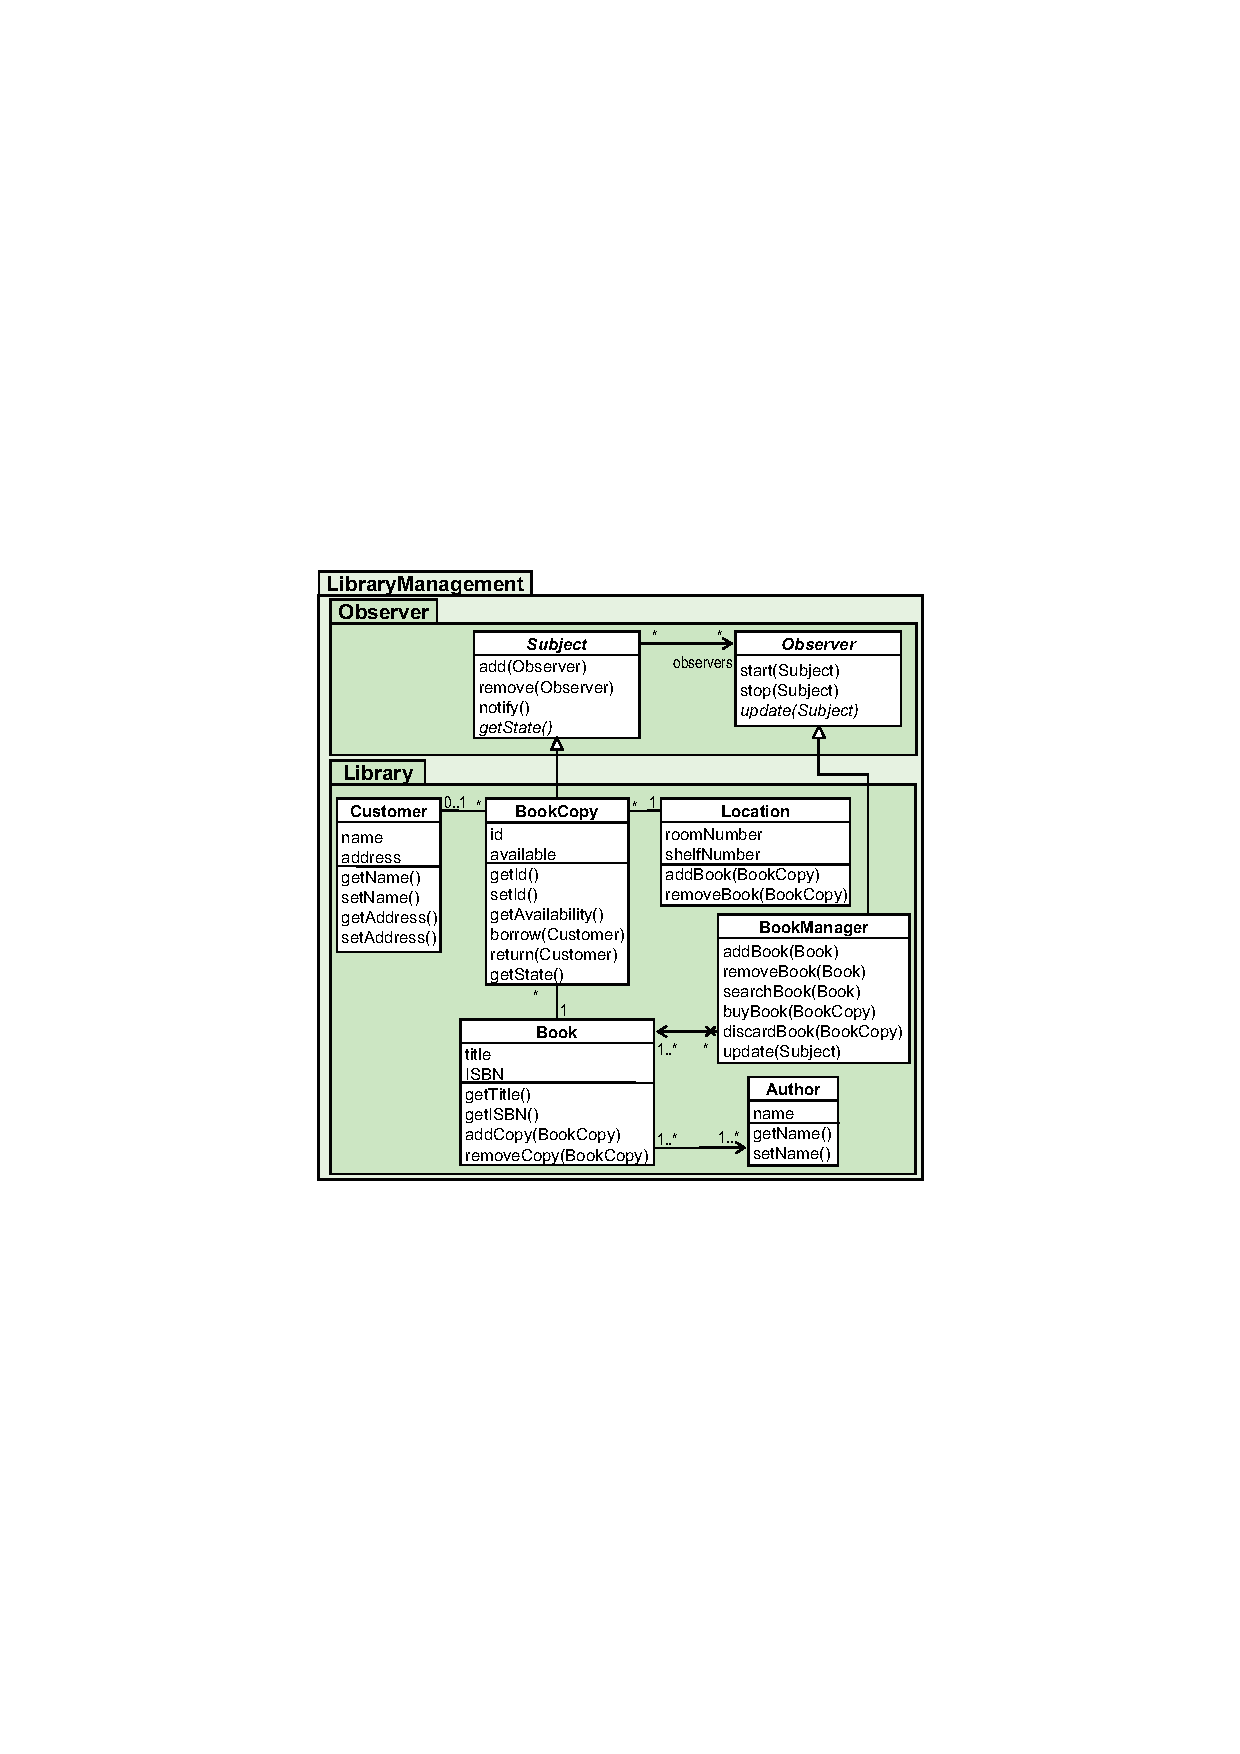
\includegraphics[width=0.7\textwidth]{figures/figure1}
	\caption{Sample figure}
	\label{fig:samplefigure_pdf}
\end{figure}


\section{Fonts}

When introducing important terms for the first time use \emph{emphasize}. For a consistent look and feel of proper names like {\cd} and {\uml{Observer}} pattern you may define macros in the main document \texttt{thesis.tex}.

\section{Code}

For short code fragments use the \textit{verbatim} environment.

\begin{verbatim}
//Start Program
System.out.println("Hello World!");
//End Program
\end{verbatim}

A much better alternative is the \textit{algorithm} environment (cf. Algorithm~\ref{alg:samplealgorithm}). This environment offers special formatting features for loops, operations and comments.

\begin{algorithm}[t]
\SetKwData{Left}{left}
\SetKwData{This}{this}
\SetKwData{Up}{up}
\SetKwFunction{Union}{Union}
\SetKwFunction{FindCompress}{FindCompress}
\SetKwInOut{Input}{input}
\SetKwInOut{Output}{output}

\Input{A bitmap $Im$ of size $w\times l$}
\Output{A partition of the bitmap}

\BlankLine

\emph{special treatment of the first line}\;
\For{$i\leftarrow 2$ \KwTo $l$}{
\emph{special treatment of the first element of line $i$}\;
\For{$j\leftarrow 2$ \KwTo $w$}{\label{forins}
\Left$\leftarrow$ \FindCompress{$Im[i,j-1]$}\;
\Up$\leftarrow$ \FindCompress{$Im[i-1,]$}\;
\This$\leftarrow$ \FindCompress{$Im[i,j]$}\;
\If(\tcp*[r]{O(\Left,\This)==1}){\Left compatible with \This}{\label{lt}
\lIf{\Left $<$ \This}{\Union{\Left,\This}}\;
\lElse{\Union{\This,\Left}\;}
}
\If(\tcp*[r]{O(\Up,\This)==1}){\Up compatible with \This}{\label{ut}
\lIf{\Up $<$ \This}{\Union{\Up,\This}}\;
\tcp{\This is put under \Up to keep tree as flat as possible}\label{cmt}
\lElse{\Union{\This,\Up}}\tcp*[r]{\This linked to \Up}\label{lelse}
}
}
\lForEach{element $e$ of the line $i$}{\FindCompress{p}}
}
\caption{Sample algorithm}\label{alg:samplealgorithm}
\end{algorithm}



%%%%%%%%%%%%%%%%%%%%%%%%%%%%%%%%%%%%%%%%%
%\chapter{References}
%\label{ch:bibliographic}
%%%%%%%%%%%%%%%%%%%%%%%%%%%%%%%%%%%%%%%%%

%\section{Literature Research}

%Information on online libraries and literature search, e.g., interesting magazines, journals, conferences, and organizations may be found at \url{http://www.big.tuwien.ac.at/teaching/info.html}.
%
%\section{BibTeX}
%
%BibTeX should be used for referencing.
%
%The LaTeX source document of this pdf document provides you with different samples for references to journals~\cite{jour:B2BServices}, conference papers~\cite{proc:TheWebMLApproach}, books~\cite{book:umlatwork}, book chapters~\cite{incoll:ErhardKonrad1992}, electronic standards~\cite{man:BPEL}, dissertations~\cite{phdthesis:manuelWimmer}, masters' theses~\cite{mast:AUMLProfile}, and web sites~\cite{misc:BIGWebsite}. The respective BibTeX entries may be found in the file \texttt{references.bib}. For administration of the BibTeX references we recommend \url{http://www.citeulike.org} or JabRef for offline administration, respectively.


%%%%%%%%%%%%%%%%%%%%%%%%%%%%%%%%%%%%%%%%%
%%% BACKMATTER %%%%%%%%%%%%%%%%%%%%%%%%%%
%%%%%%%%%%%%%%%%%%%%%%%%%%%%%%%%%%%%%%%%%

\appendix

\bibliographystyle{plain}
\bibliography{references}

\end{document}
